\documentclass[aspectratio=169, 10pt]{beamer}
\usepackage{fontspec}
\usepackage{graphicx}
\usepackage{amsmath, amssymb}
\usepackage{booktabs}
\usepackage{xcolor}

% Pirsch Analytics Design Tokens
\definecolor{CreamPaper}{HTML}{F8F5ED}
\definecolor{InkBlack}{HTML}{000000}
\definecolor{GraphiteMuted}{HTML}{707070}
\definecolor{SunshineYellow}{HTML}{FFDA6E}
\definecolor{MintGreen}{HTML}{15803D}
\definecolor{AlertRed}{HTML}{DC2626}
\definecolor{WarnAmber}{HTML}{D97706}
\definecolor{WhitePure}{HTML}{FFFFFF}

% Beamer Theme Configuration
\setbeamercolor{normal text}{fg=InkBlack, bg=CreamPaper}
\setbeamercolor{structure}{fg=InkBlack}
\setbeamercolor{title}{fg=InkBlack}
\setbeamercolor{frametitle}{fg=InkBlack, bg=CreamPaper}
\setbeamercolor{block title}{fg=InkBlack, bg=SunshineYellow}
\setbeamercolor{block body}{fg=InkBlack, bg=WhitePure}
\setbeamercolor{block title alerted}{fg=WhitePure, bg=AlertRed}
\setbeamercolor{block body alerted}{fg=InkBlack, bg=WhitePure}

\setbeamertemplate{navigation symbols}{}
\setbeamertemplate{frametitle}{
    \nointerlineskip
    \begin{beamercolorbox}[sep=0.35cm,wd=\paperwidth]{frametitle}
        {\large\textbf{\insertframetitle}} \hfill \scriptsize \textcolor{GraphiteMuted}{\insertframesubtitle}
    \end{beamercolorbox}
    \vspace{-0.1cm}
    \textcolor{InkBlack}{\rule{\paperwidth}{0.8pt}}
}
\setbeamertemplate{footline}{
    \leavevmode
    \textcolor{InkBlack}{\rule{\paperwidth}{0.8pt}}
    \hbox{
        \begin{beamercolorbox}[wd=.6\paperwidth,ht=2.5ex,dp=1.125ex,leftskip=.3cm]{normal text}
            \scriptsize \textbf{ECDR Week 3:} Mathematical Foundations \& Feasibility Study
        \end{beamercolorbox}
        \begin{beamercolorbox}[wd=.4\paperwidth,ht=2.5ex,dp=1.125ex,rightskip=.3cm,right]{normal text}
            \scriptsize \insertframenumber{} / \inserttotalframenumber
        \end{beamercolorbox}
    }
    \vskip2pt
}

\title{\textbf{Báo Cáo Nghiên Cứu Tuần 3: ECDR}}
\subtitle{Mathematical Foundations, Certified Decision Reuse \& Experimental Feasibility}
\author{\textbf{Nhóm Nghiên Cứu ECDR} \\ Mô hình tham chiếu: Frozen SmallCNN1D (K=12) trên HAPT}
\date{03 Tháng 11, 2026}

\begin{document}

% SLIDE 0: TITLE
\begin{frame}
    \titlepage
\end{frame}

% SLIDE 01: DUAL TRACK
\begin{frame}{Từ Phân Loại CNN Đến Certified Decision Reuse}{Part A. Research Context • Slide 01}
    \begin{columns}
        \begin{column}{0.55\textwidth}
            \centering
            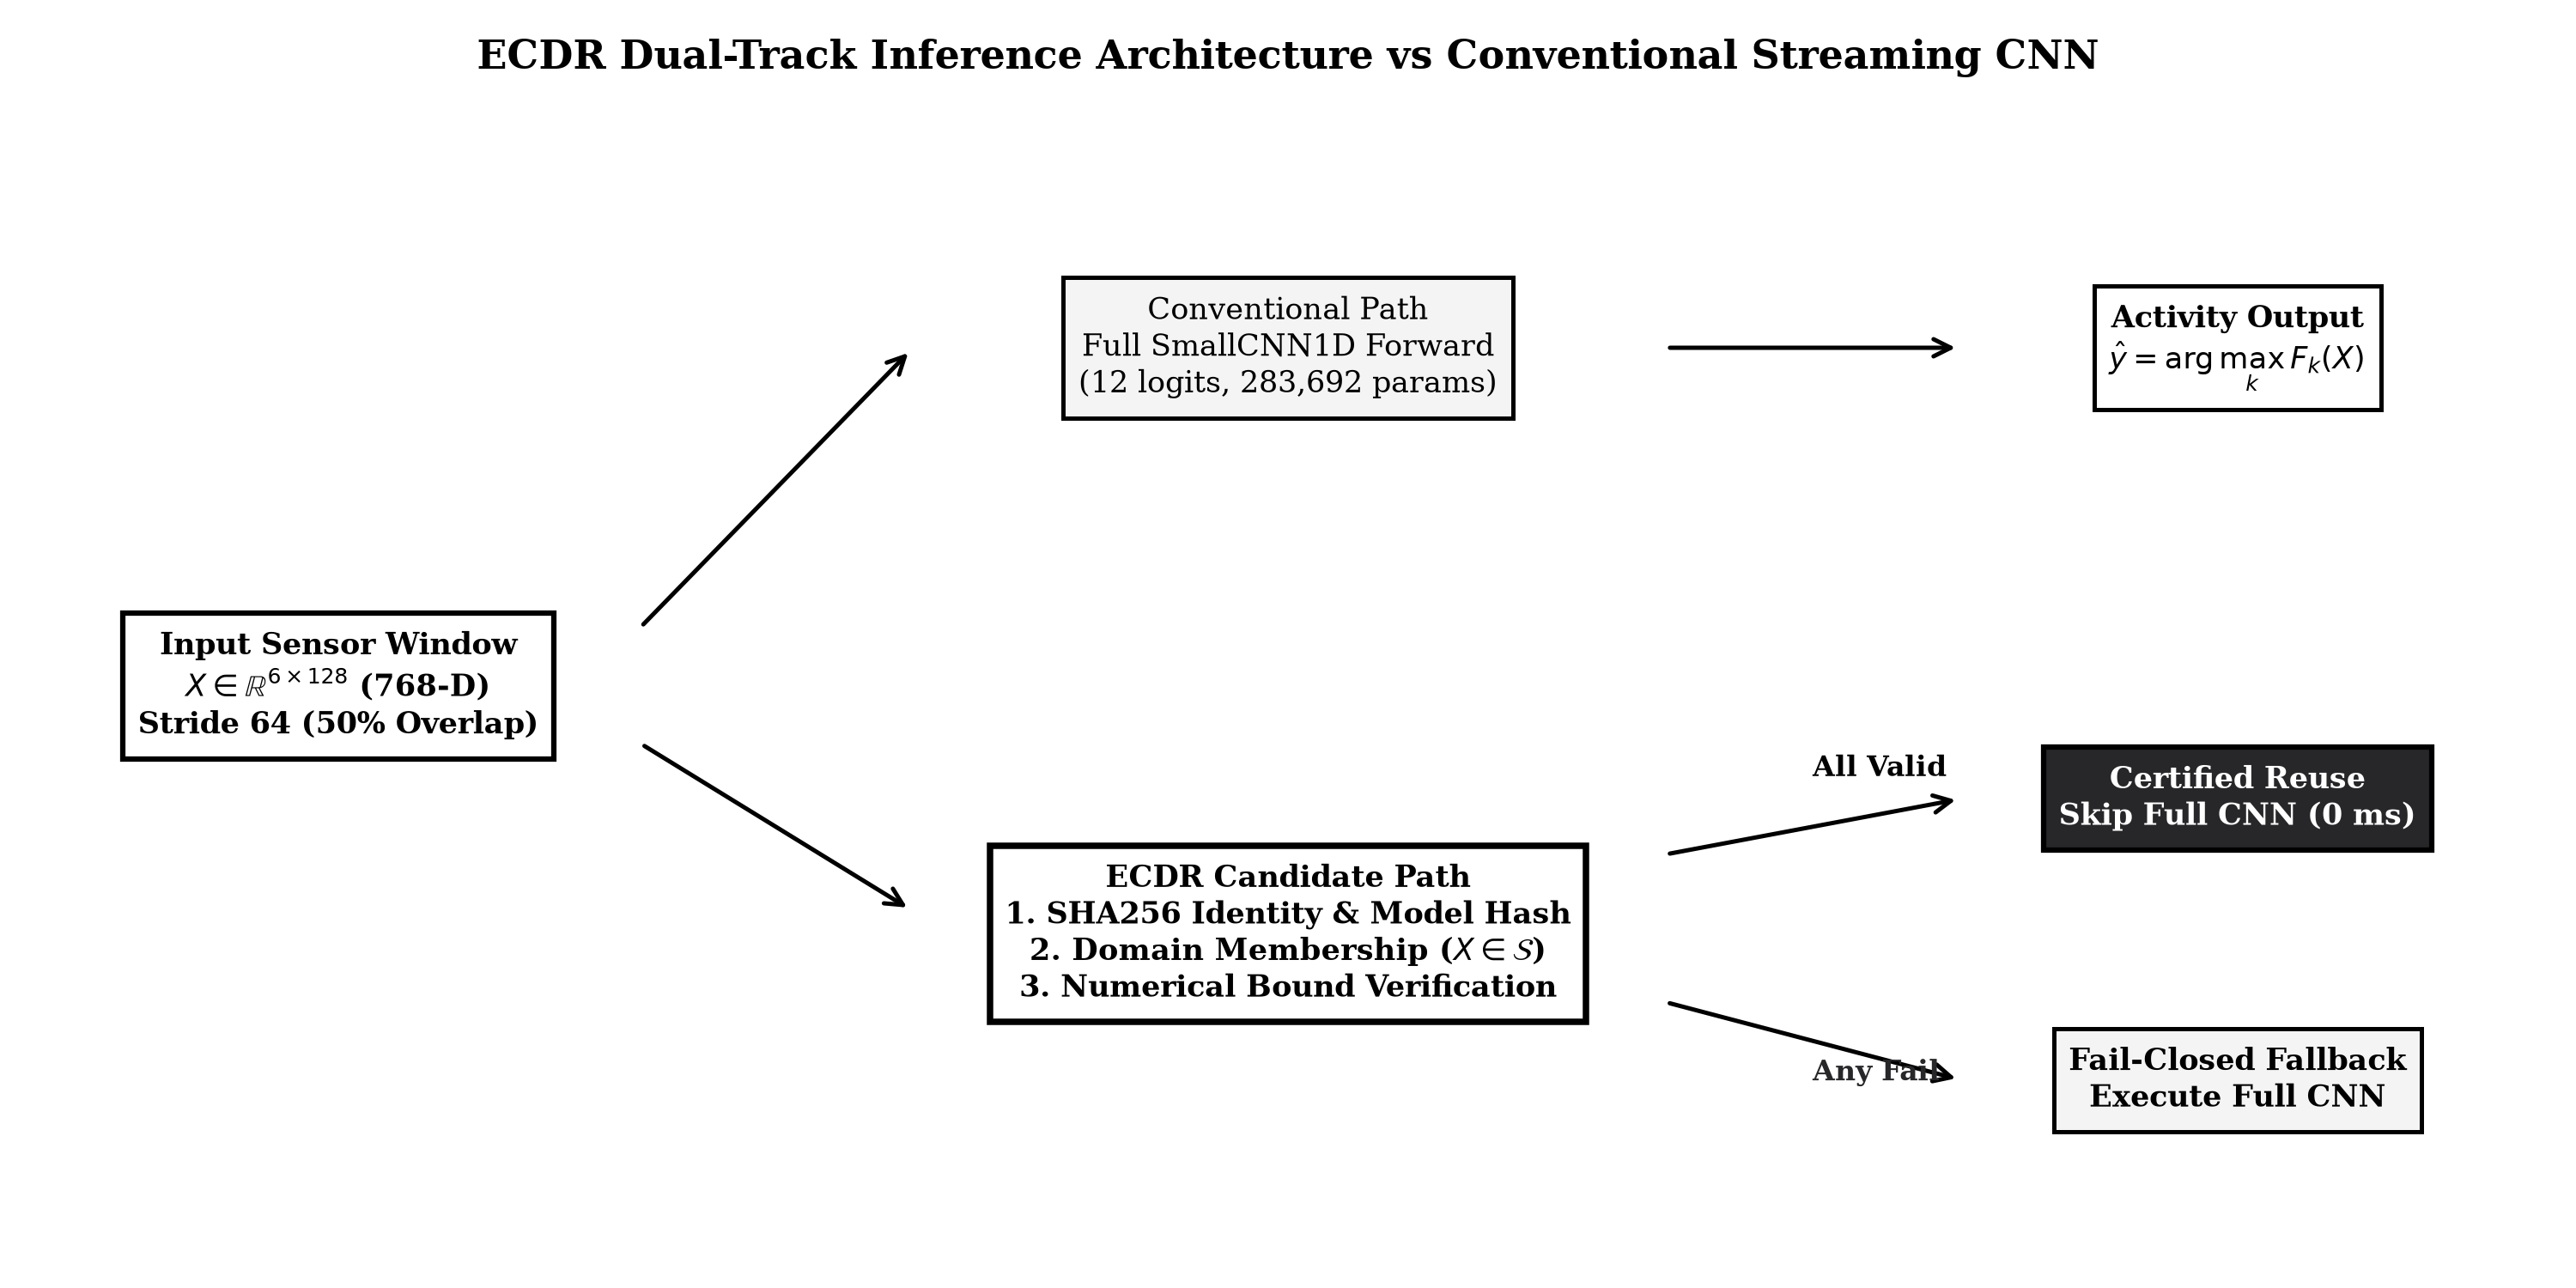
\includegraphics[width=\textwidth]{assets/fig01_dual_track.png}
        \end{column}
        \begin{column}{0.43\textwidth}
            \begin{block}{\textbf{3 Bất Biến Nghiên Cứu Không Nhân Nhượng}}
                \begin{itemize}
                    \item \textbf{1. Không sửa nhãn:} Giữ nguyên 12 nhãn thực tế HAPT.
                    \item \textbf{2. Không sửa weights:} 283.692 params float32 bất biến.
                    \item \textbf{3. Không đánh đổi accuracy:} Chỉ reuse khi có chứng nhận toán học cùng winner 100\%.
                \end{itemize}
            \end{block}
            \vspace{0.2cm}
            \alert{\textbf{Nguyên tắc Fail-Closed:}} Mọi sự cố xác thực đều kích hoạt fallback 100\% về CNN.
        \end{column}
    \end{columns}
\end{frame}

% SLIDE 02: FROZEN CONTRACT
\begin{frame}{Hợp Đồng Bất Biến Của Frozen Reference}{Part A. Research Context • Slide 02}
    \begin{columns}
        \begin{column}{0.48\textwidth}
            \begin{block}{\textbf{Toán Tử Toàn Phần: $F(X) = f_\theta(N(X))$}}
                \small
                \begin{itemize}
                    \item \textbf{Input:} $(B, 6, 128)$ cảm biến float32.
                    \item \textbf{Output:} $(B, 12)$ logits.
                    \item \textbf{Chuẩn hóa $N(X)$:} Z-score cố định (SHA256: \texttt{aa8e1cc2...}).
                    \item \textbf{Checkpoint:} Seed 43, Epoch 8 (SHA256: \texttt{8ffc5dd8...}).
                    \item \textbf{Graph:} 3 Conv1D-BN-ReLU, 2 MaxPool, Flatten-MLP.
                \end{itemize}
            \end{block}
        \end{column}
        \begin{column}{0.48\textwidth}
            \begin{block}{\textbf{Tập Dữ Liệu \& Môi Trường}}
                \small
                \begin{itemize}
                    \item \textbf{Hardware/OS:} Linux, CPU 1-thread, PyTorch 2.14.
                    \item \textbf{Test stream:} 5.053 cửa sổ (19 recordings).
                    \item \textbf{Supervised subset:} 3.572 cửa sổ.
                \end{itemize}
            \end{block}
            \vspace{0.2cm}
            \begin{alertblock}{\textbf{Lưu ý Bản Quyền Hợp Đồng}}
                Chứng chỉ chỉ có hiệu lực với đúng toán tử $F(X)$. Bất kỳ thay đổi nào ở weights hay normalization đều vô hiệu hóa certificate.
            \end{alertblock}
        \end{column}
    \end{columns}
\end{frame}

% SLIDE 03: RQs & DELIVERABLES
\begin{frame}{Câu Hỏi Nghiên Cứu \& Sản Phẩm Bàn Giao}{Part A. Research Context • Slide 03}
    \begin{columns}
        \begin{column}{0.5\textwidth}
            \small
            \begin{tabular}{lp{4.8cm}}
                \toprule
                \textbf{RQ} & \textbf{Nội dung kiểm chứng Tuần 3} \\
                \midrule
                \textbf{RQ1} & Tái xác nhận mô hình khóa; khớp 100\% predictions trên 5.053 cửa sổ test. \\
                \textbf{RQ2} & Xây dựng verifier IBP trên actual graph; tính cận margin 11 lớp. \\
                \textbf{RQ3} & Đo đạc thời gian 4 luồng replay thực tế; đo latency build, membership, fallback. \\
                \bottomrule
            \end{tabular}
        \end{column}
        \begin{column}{0.46\textwidth}
            \begin{block}{\textbf{5 Sản Phẩm Bàn Giao Kỹ Thuật}}
                \footnotesize
                \begin{enumerate}
                    \item \textbf{Report A (26p):} Mathematical Foundations.
                    \item \textbf{Report B (33p):} Mathematics Explained.
                    \item \textbf{Verifier Code:} \texttt{ecdr/week3\_verifier.py}.
                    \item \textbf{Experimental Traces:} JSON \& CSV traces.
                    \item \textbf{Test Suite:} 93/93 tests unit/regression PASS.
                \end{enumerate}
            \end{block}
        \end{column}
    \end{columns}
\end{frame}

% SLIDE 04: HYPOTHESIS MAP
\begin{frame}{Phân Loại 24 Giả Thuyết Khoa Học (H01–H24)}{Part A. Research Context • Slide 04}
    \begin{columns}
        \begin{column}{0.55\textwidth}
            \centering
            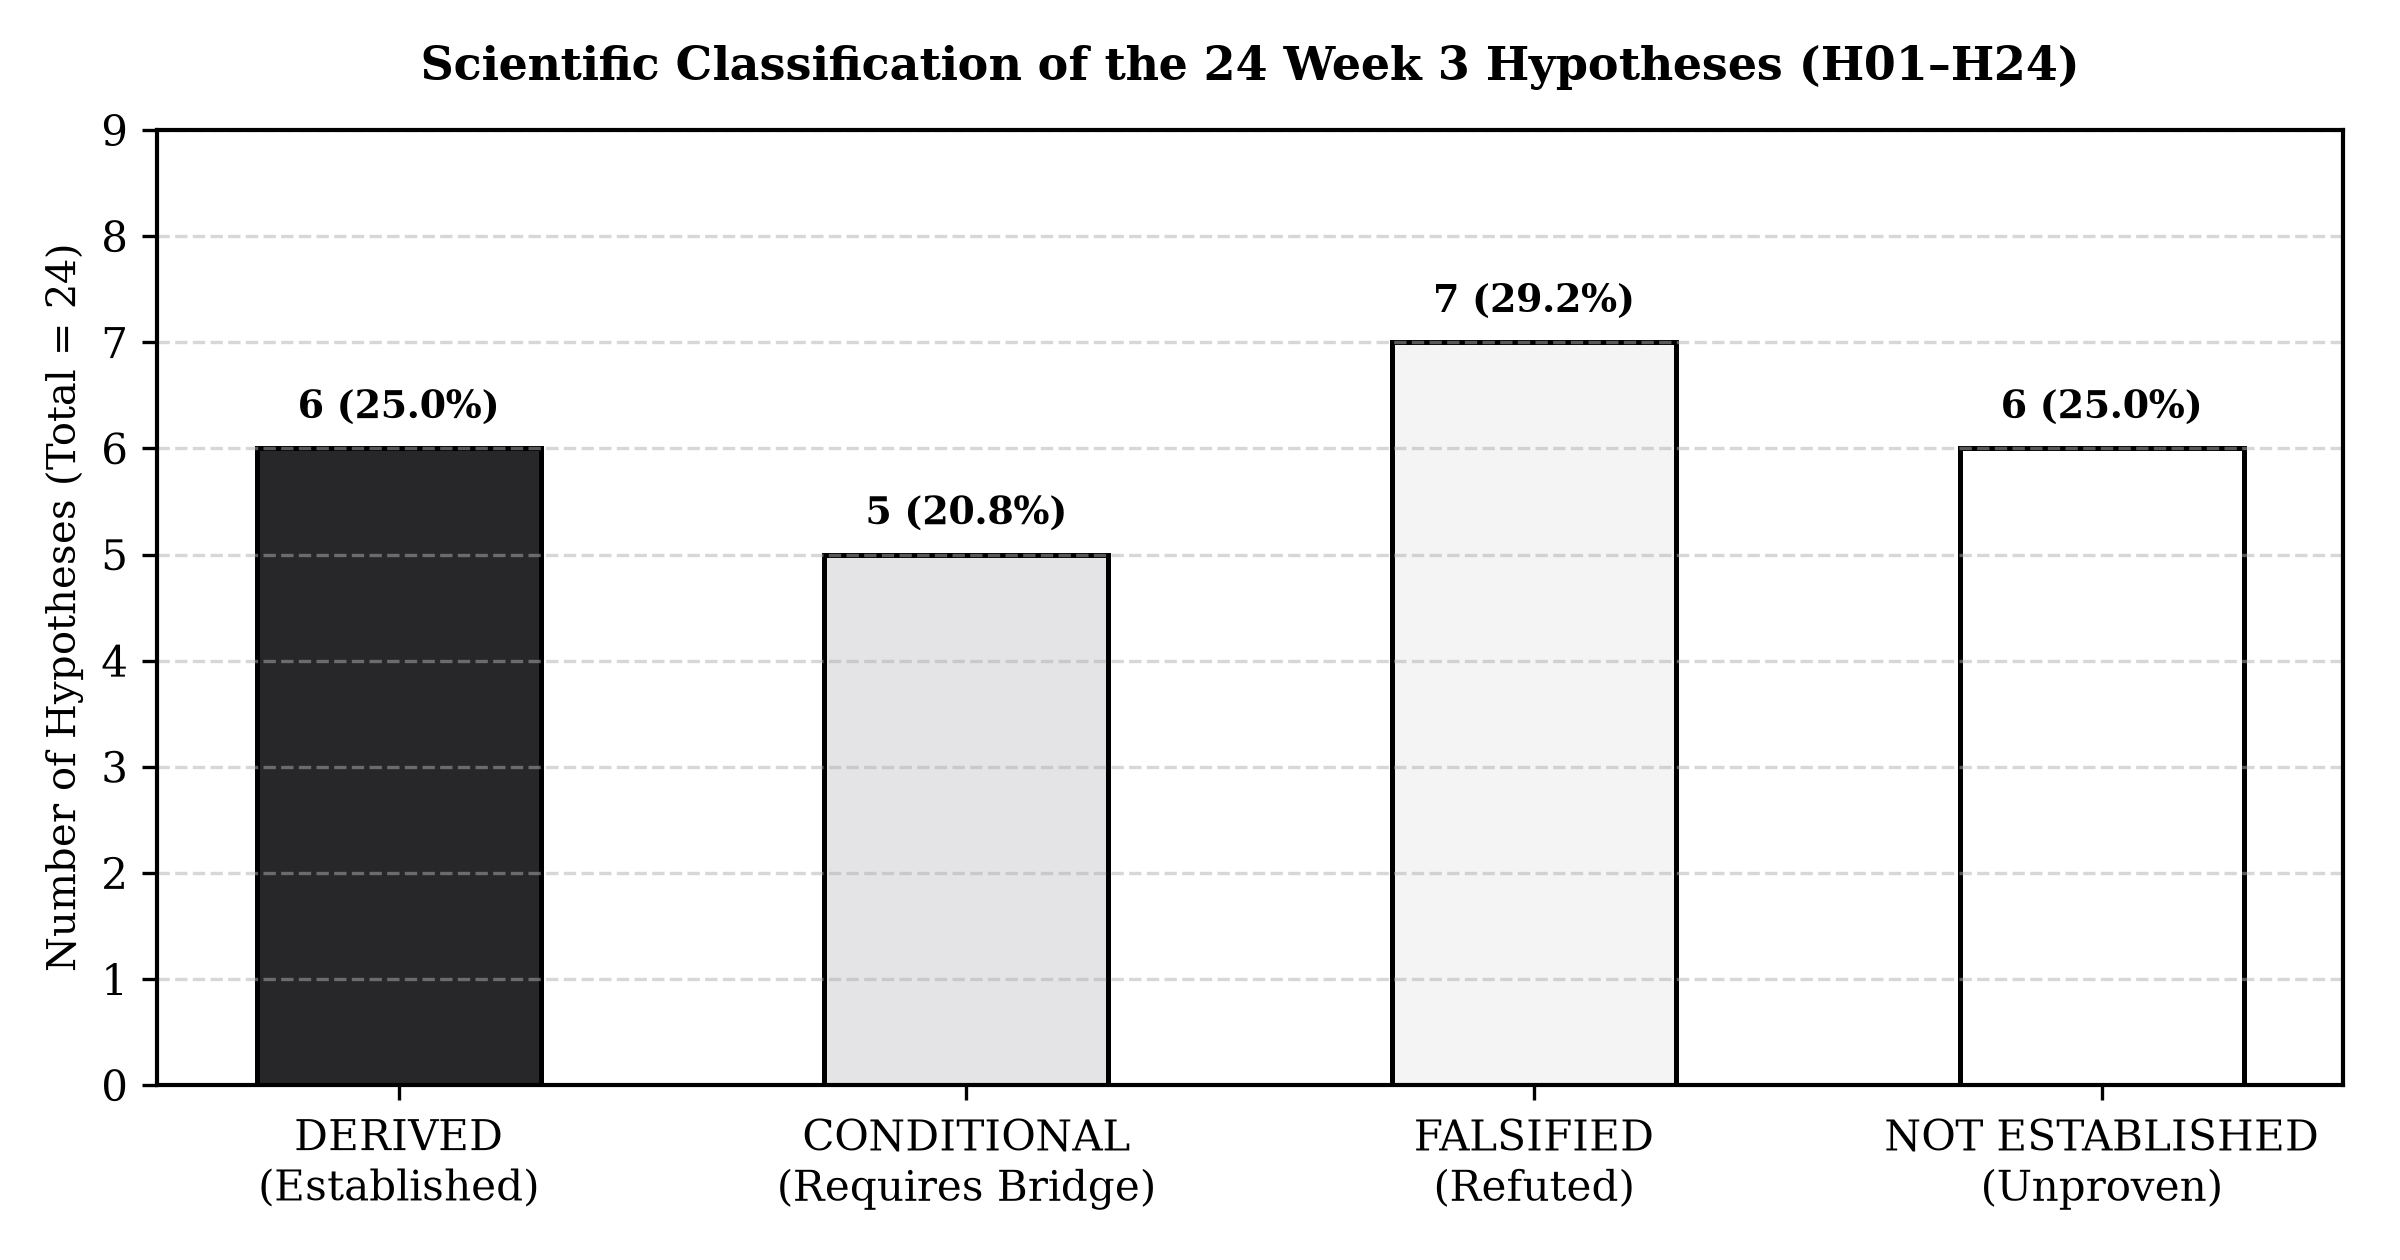
\includegraphics[width=\textwidth]{assets/fig07_hypothesis_status_breakdown.png}
        \end{column}
        \begin{column}{0.42\textwidth}
            \begin{alertblock}{\textbf{Mệnh Đề Nghiên Cứu Cốt Lõi}}
                $$\text{Soundness} \not\implies \text{Coverage} \not\implies \text{Cost Saving}$$
            \end{alertblock}
            \footnotesize
            \begin{itemize}
                \item \textbf{Soundness:} Cận margin hợp lệ trong miền.
                \item \textbf{Coverage:} Miền chứa được dữ liệu mới.
                \item \textbf{Cost Saving:} Tiết kiệm thời gian ròng.
            \end{itemize}
            \vspace{0.1cm}
            Bắt buộc cả 3 điều kiện đồng thời thỏa mãn mới đạt được speedup.
        \end{column}
    \end{columns}
\end{frame}

% SLIDE 05: SENSOR OVERLAP
\begin{frame}{Không Gian Cảm Biến 768 Chiều \& Temporal Overlap}{Part B. Mathematical Foundations • Slide 05}
    \begin{columns}
        \begin{column}{0.55\textwidth}
            \centering
            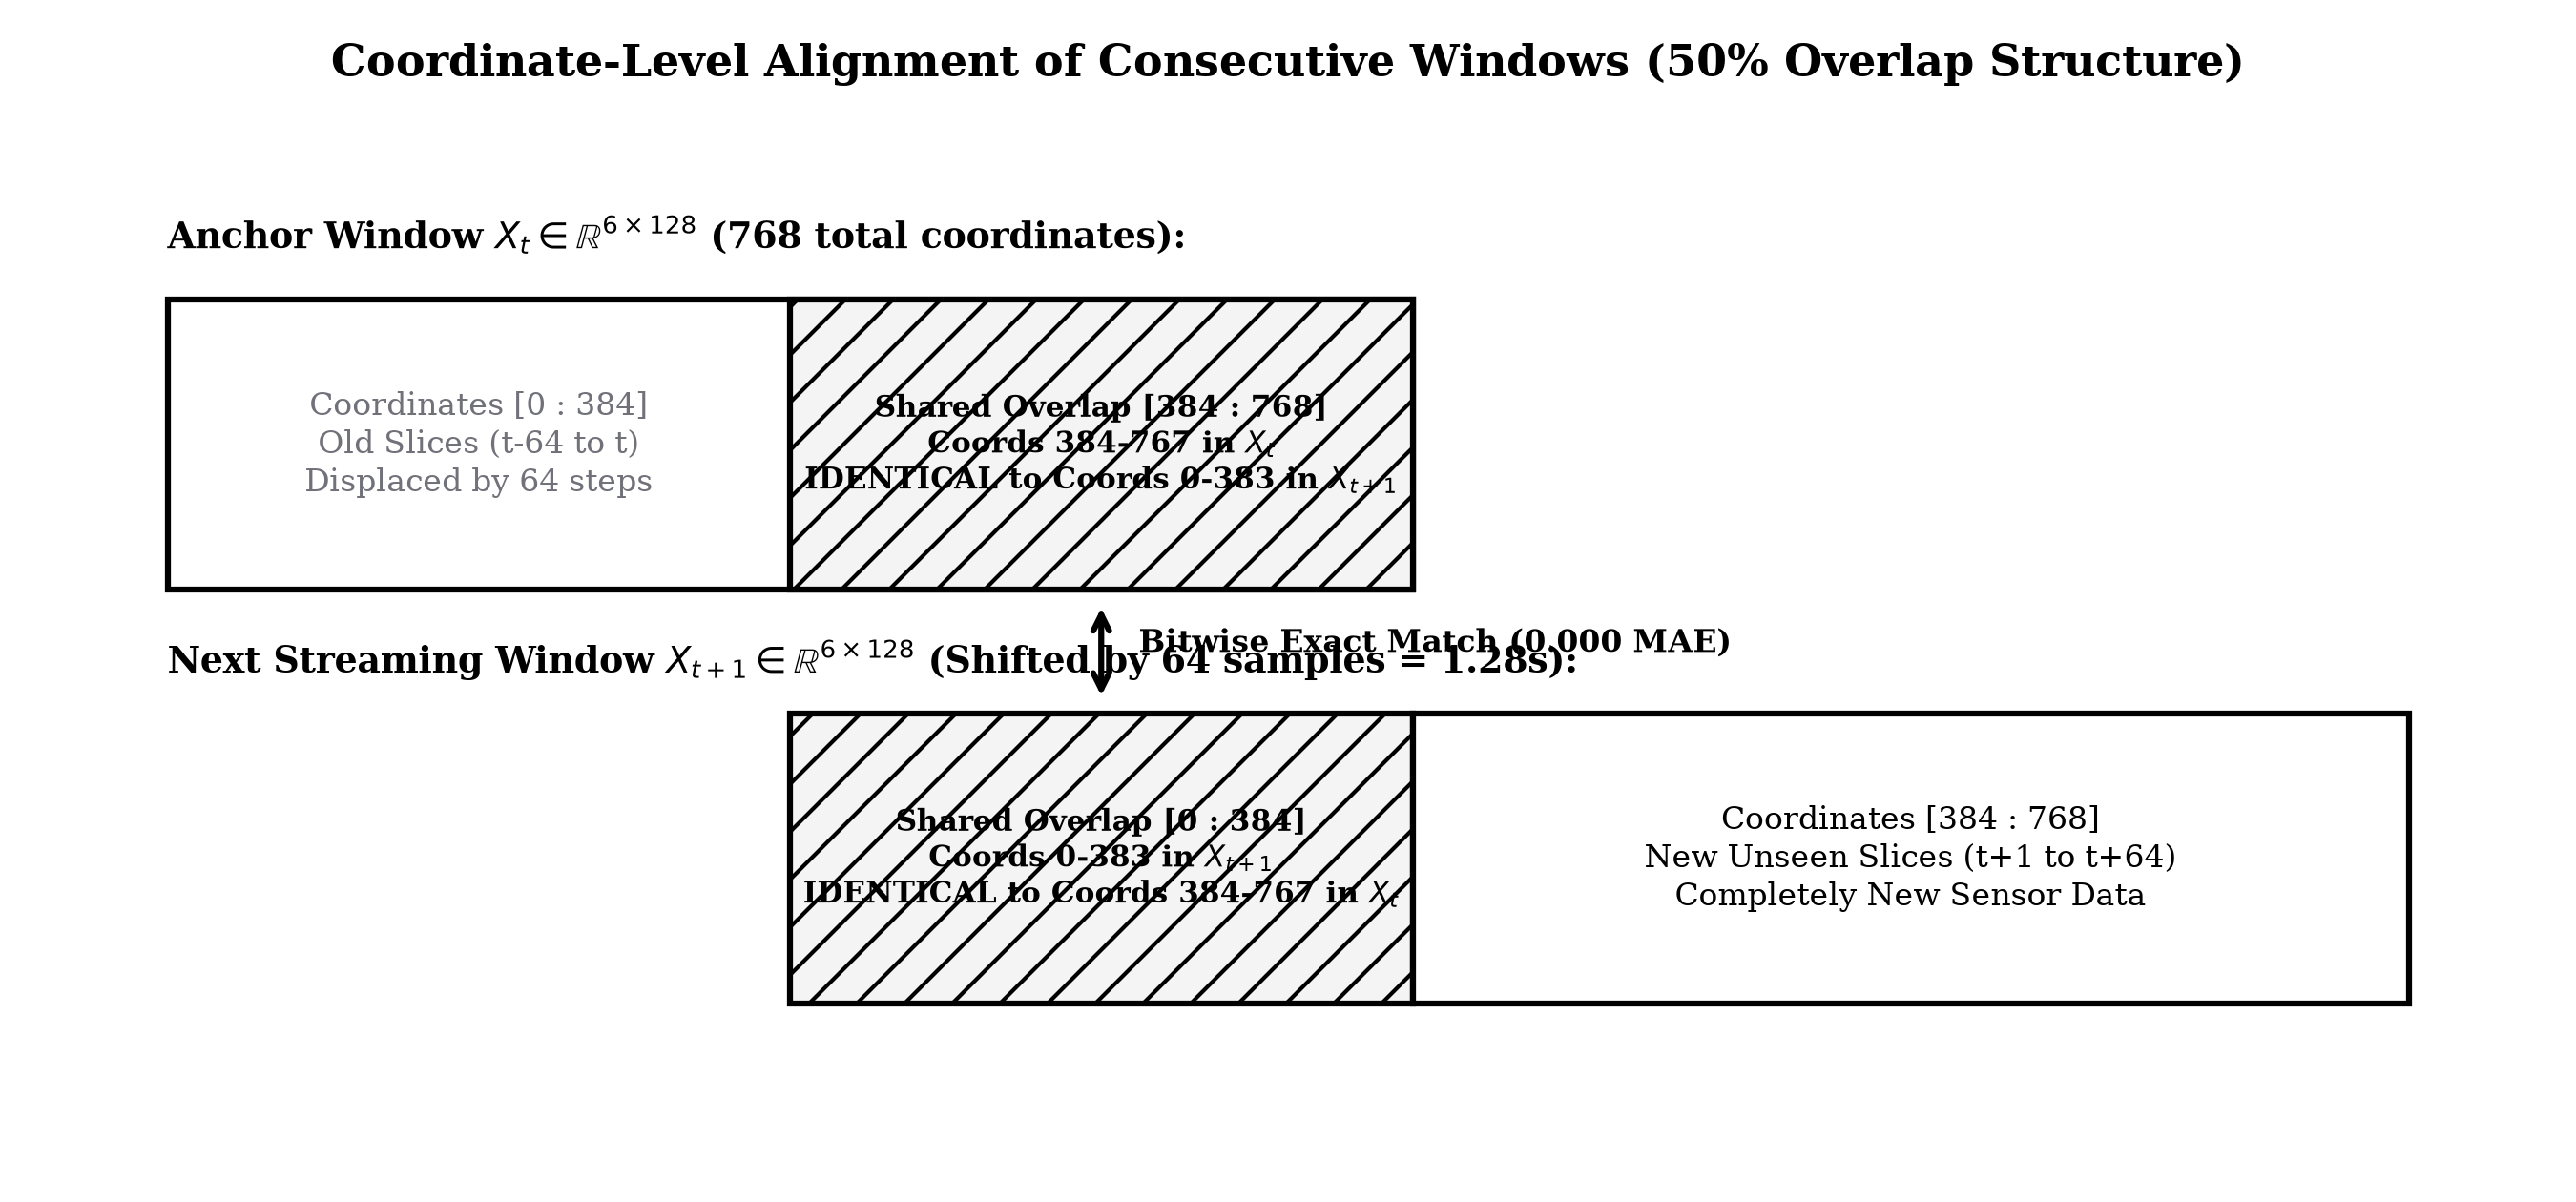
\includegraphics[width=\textwidth]{assets/fig02_overlap_geometry.png}
        \end{column}
        \begin{column}{0.42\textwidth}
            \begin{block}{\textbf{Phân Rã Tọa Độ Vật Lý}}
                \footnotesize
                \begin{itemize}
                    \item $X \in \mathbb{R}^{6 \times 128} \implies 768$ tọa độ thực.
                    \item Stride 64 samples (50\% overlap):
                    \begin{itemize}
                        \item \textbf{384 tọa độ cố định:} Dữ liệu từ cửa sổ trước.
                        \item \textbf{384 tọa độ tự do:} Dữ liệu mới thu thập.
                    \end{itemize}
                \end{itemize}
            \end{block}
            \vspace{0.1cm}
            \textbf{Fixed-Overlap Wave Domain:} Khóa cứng 384 tọa độ đã biết, giảm bậc tự do từ 768 xuống 384!
        \end{column}
    \end{columns}
\end{frame}

% SLIDE 06: MARGIN THEOREM
\begin{frame}{Khoảng Cách Quyết Định \& Định Lý Chứng Nhận}{Part B. Mathematical Foundations • Slide 06}
    \begin{columns}
        \begin{column}{0.52\textwidth}
            \begin{block}{\textbf{Định Lý Chứng Nhận (Theorem H05)}}
                Cho trusted anchor $X^r$, winner $c = \arg\max_k F_k(X^r)$.
                Với mọi lớp đối thủ $j \neq c$, margin:
                $$g_{cj}(X) = F_c(X) - F_j(X)$$
                Nếu tồn tại miền $S$ thỏa mãn:
                $$\boxed{\min_{j \neq c} \underline{g}_{cj}(S) > 0}$$
                thì $\forall X \in S$, CNN giữ nguyên winner $c$.
            \end{block}
        \end{column}
        \begin{column}{0.44\textwidth}
            \small
            \begin{tabular}{llc}
                \toprule
                \textbf{Đại lượng} & \textbf{Ý nghĩa} & \textbf{Reuse?} \\
                \midrule
                Point margin & Margin tại 1 điểm & \textcolor{AlertRed}{\textbf{Không}} \\
                Regional min & Cực tiểu thực tế & \textcolor{MintGreen}{\textbf{Có}} \\
                Valid lower bound & Cận dưới bảo thủ & \textcolor{MintGreen}{\textbf{Có}} \\
                Diagnostic est. & Ước lượng float64 & \textcolor{WarnAmber}{\textbf{Chưa}} \\
                \bottomrule
            \end{tabular}
            \vspace{0.2cm}
            \footnotesize
            Chỉ cần 1 trong 11 cận dưới $\le 0$, chứng chỉ bị từ chối ngay lập tức.
        \end{column}
    \end{columns}
\end{frame}

% SLIDE 07: IBP ON ACTUAL CNN
\begin{frame}{Lan Truyền Khoảng (IBP) Trên SmallCNN1D Thật}{Part B. Mathematical Foundations • Slide 07}
    \begin{columns}
        \begin{column}{0.5\textwidth}
            \begin{block}{\textbf{Quy Tắc Lan Truyền Khoảng Toán Tử}}
                \footnotesize
                \begin{itemize}
                    \item \textbf{Affine ($Wx+b$):} $\underline{y} = W^+ \underline{x} + W^- \overline{x} + b$.
                    \item \textbf{Conv1D:} Áp dụng signed weights theo kernel.
                    \item \textbf{BatchNorm(eval):} Affine channel-wise cố định.
                    \item \textbf{ReLU:} $[\max(0, \underline{x}), \max(0, \overline{x})]$.
                    \item \textbf{MaxPool1D:} Lấy min của lower, max của upper.
                    \item \textbf{Flatten:} Định hình lại tensor, giữ khoảng.
                \end{itemize}
            \end{block}
        \end{column}
        \begin{column}{0.46\textwidth}
            \begin{block}{\textbf{Direct Final Margin Bounds}}
                \footnotesize
                Tạo vector chênh lệch $W_{cj} = W_c - W_j$ ở Linear cuối:
                $$\underline{g}_{cj} = W_{cj}^+ \underline{h} + W_{cj}^- \overline{h} + (b_c - b_j)$$
            \end{block}
            \vspace{0.1cm}
            \alert{\textbf{Ưu thế kỹ thuật:}} Triệt tiêu hoàn toàn dependency loss giữa 2 logits cạnh tranh ở tầng output!
        \end{column}
    \end{columns}
\end{frame}

% SLIDE 08: DOMAIN DESIGN
\begin{frame}{Thiết Kế Miền Ứng Viên: Diagonal Box vs Wave Domain}{Part B. Mathematical Foundations • Slide 08}
    \begin{columns}
        \begin{column}{0.48\textwidth}
            \begin{block}{\textbf{Diagonal Box Domain (768-D)}}
                \small
                \begin{itemize}
                    \item Cả 768 tọa độ biến thiên độc lập.
                    \item Tâm: Normalized anchor $N(X^r)$.
                    \item Khoảng: $[X^0 - \rho, X^0 + \rho]$.
                    \item Kiểm tra membership: $\Theta(m)$, $m=768$.
                \end{itemize}
            \end{block}
        \end{column}
        \begin{column}{0.48\textwidth}
            \begin{block}{\textbf{Fixed-Overlap Wave Domain (384-D)}}
                \small
                \begin{itemize}
                    \item 384 tọa độ đầu khóa cứng bằng suffix cũ.
                    \item Tâm: Continuation rule $[X^r[64:], X^r[64:]]$.
                    \item Chỉ 384 tọa độ mới biến thiên trong $\rho$.
                \end{itemize}
            \end{block}
        \end{column}
    \end{columns}
    \vspace{0.3cm}
    \centering
    \alert{\textbf{Lưu ý quan trọng:}} Continuation rule không phải tiên tri tương lai. Nếu tín hiệu mới lệch ra ngoài, membership lập tức trả về false. Giảm 384 chiều không đồng nghĩa giảm 50\% chi phí CNN.
\end{frame}

% SLIDE 09: FEATURE ALIGNMENT H13
\begin{frame}{Định Lý Căn Chỉnh Đặc Trưng (H13) Khớp Bitwise 100\%}{Part B. Mathematical Foundations • Slide 09}
    \begin{columns}
        \begin{column}{0.55\textwidth}
            \centering
            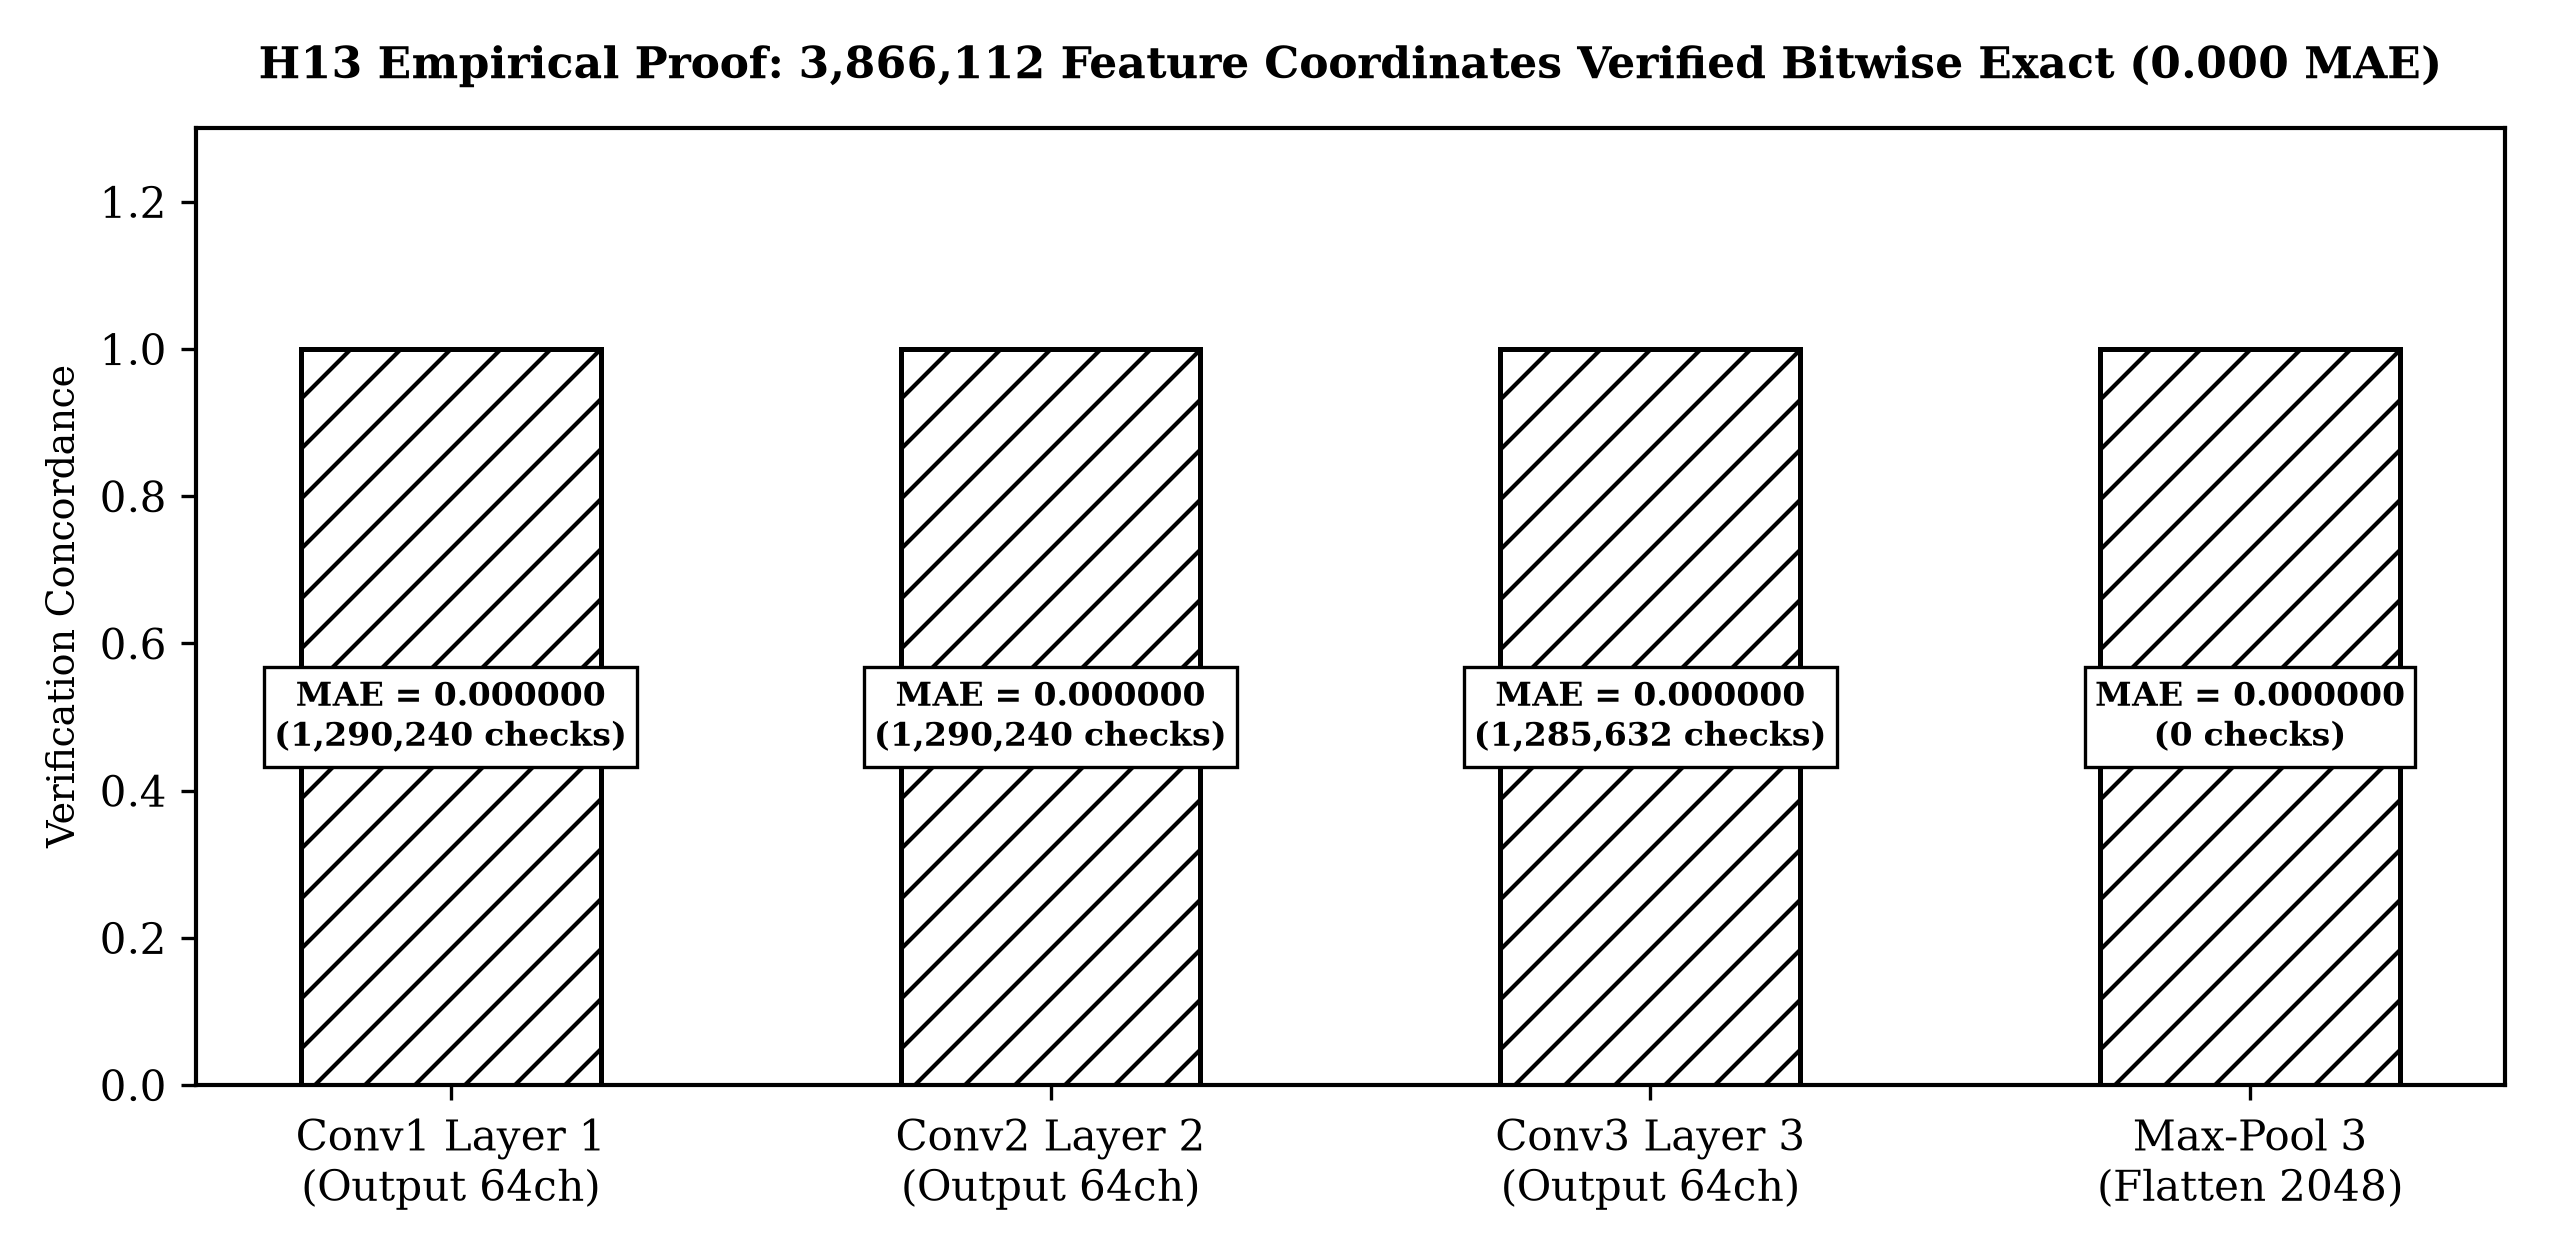
\includegraphics[width=\textwidth]{assets/fig03_h13_feature_alignment.png}
        \end{column}
        \begin{column}{0.42\textwidth}
            \begin{block}{\textbf{Định Lý Căn Chỉnh Toán Học}}
                \footnotesize
                Receptive field $[4j-8, 4j+11]$ (độ rộng 20, jump 4).
                Tại 12 vị trí nội bộ $j \in [2, 13]$:
                $$H_j(X_{\text{new}}) = H_{j+16}(X_{\text{previous}})$$
            \end{block}
            \vspace{0.1cm}
            \begin{alertblock}{\textbf{Kiểm Chứng Độc Lập}}
                \footnotesize
                5.034 cặp adjacent windows $\times$ 12 vị trí $\times$ 64 channels = \textbf{3.866.112 phép kiểm tra bitwise match (sai số = 0.0)}.
            \end{alertblock}
            \tiny
            (Tầng Flatten-MLP nhạy vị trí khiến logits vẫn biến đổi).
        \end{column}
    \end{columns}
\end{frame}

% SLIDE 10: NUMERICAL SOUNDNESS
\begin{frame}{Bảo Đảm Số Học: Vì Sao Proof Số Thực Chưa Đủ Cho Float32?}{Part B. Mathematical Foundations • Slide 10}
    \begin{columns}
        \begin{column}{0.48\textwidth}
            \begin{block}{\textbf{3 Cấp Độ Hợp Lệ}}
                \small
                \begin{enumerate}
                    \item \textbf{Level 1: Mathematical Validity} \\ Chứng minh trên trường số thực $\mathbb{R}$.
                    \item \textbf{Level 2: Executable Numerical} \\ Cận bao bọc backend float32 (IEEE-754, sai số làm tròn).
                    \item \textbf{Level 3: Finite Test Consistency} \\ Unit tests trên tập mẫu hữu hạn.
                \end{enumerate}
            \end{block}
        \end{column}
        \begin{column}{0.48\textwidth}
            \begin{alertblock}{\textbf{Bác Bỏ Giả Thuyết H22 (Falsified)}}
                \small
                "Chứng minh toán học trên số thực tự động đúng cho thực thi float32" là \textbf{SAI}.
            \end{alertblock}
            \vspace{0.2cm}
            \small
            Verifier chạy PyTorch float64 chỉ làm giảm sai số, nhưng chưa có directed rounding để bao bọc hoàn toàn float32.
            \\ $\implies$ \textbf{Khóa fail-closed:} \texttt{formal\_reuse\_enabled = False}.
        \end{column}
    \end{columns}
\end{frame}

% SLIDE 11: VERIFIER ARCHITECTURE
\begin{frame}{Kiến Trúc Bộ Verifier Trên Actual Graph}{Part C. System Implementation • Slide 11}
    \begin{columns}
        \begin{column}{0.5\textwidth}
            \begin{block}{\textbf{Các Thực Thể Phần Mềm (\texttt{week3\_verifier.py})}}
                \footnotesize
                \begin{itemize}
                    \item \texttt{FrozenK12Reference}: Khóa weights, normalization, state SHA256.
                    \item \texttt{CandidateBox}: Lưu trữ cận trên/dưới bất biến.
                    \item \texttt{ActualGraphIBP}: Snapshot float64, lan truyền khoảng qua Conv-BN-ReLU-MaxPool-Linear.
                    \item \texttt{ConditionalCertificate}: Lưu 11 margins và cờ numerical status.
                    \item \texttt{RuntimeGate}: Điều phối streaming và fallback.
                \end{itemize}
            \end{block}
        \end{column}
        \begin{column}{0.46\textwidth}
            \begin{alertblock}{\textbf{Triển Khai Đồ Thị Thật}}
                \footnotesize
                Verifier được tích hợp trực tiếp vào đồ thị 12 lớp thật của mô hình khóa, loại bỏ hoàn toàn các mô hình đồ chơi Conv-valid hay GAP lịch sử.
            \end{alertblock}
            \vspace{0.2cm}
            \footnotesize
            Toàn bộ logic membership, lifecycle và fallback đã được cài đặt và kiểm thử hoàn chỉnh.
        \end{column}
    \end{columns}
\end{frame}

% SLIDE 12: LIFECYCLE & FAIL-CLOSED
\begin{frame}{Vòng Đời Chứng Chỉ \& Chống Certificate Drift (H15)}{Part C. System Implementation • Slide 12}
    \begin{block}{\textbf{Quy Trình 7 Bước Kiểm Soát Tại RuntimeGate}}
        \footnotesize
        \begin{enumerate}
            \item Check Model Checkpoint SHA256 $\implies$ Khớp tuyệt đối.
            \item Check Preprocessing Z-score SHA256 $\implies$ Khớp tuyệt đối.
            \item Check Recording Continuity $\implies$ Tự động reset khi chuyển bản ghi.
            \item Check Anchor Age $\le 128$ steps $\implies$ Hết hạn tự động fallback.
            \item Check Cả 11 Cận Margin $\underline{g}_{cj}(S) > 0 \implies$ Đồng thời dương.
            \item Check Domain Membership ($X \in S$) $\implies$ Thuộc miền.
            \item Check Executable Numerical Guarantee $\implies$ Có chứng nhận số học.
        \end{enumerate}
    \end{block}
    \vspace{0.1cm}
    \alert{\textbf{Chống Trôi Dạt (Certificate Drift - H15):}} Quyết định reuse không bao giờ được phép làm anchor mới!
\end{frame}

% SLIDE 13: CROWN / LIRPA PROBE
\begin{frame}{Khảo Sát auto-LiRPA / CROWN: Cơ Hội \& Giới Hạn}{Part C. System Implementation • Slide 13}
    \small
    \begin{tabular}{llp{5.5cm}}
        \toprule
        \textbf{Phép thử nghiệm} & \textbf{Kết quả} & \textbf{Nguyên nhân kỹ thuật} \\
        \midrule
        Import auto-LiRPA 0.8.0 & \textcolor{MintGreen}{\textbf{PASS}} & Thư viện có sẵn trong môi trường. \\
        Version contract & \textcolor{WarnAmber}{\textbf{WARN}} & Không tương thích PyTorch 2.14.1+cpu. \\
        Convert native CNN1D & \textcolor{AlertRed}{\textbf{FAIL}} & Lỗi \texttt{IndexError} trên toán tử MaxPool1D. \\
        Convert surrogate 2D ($H=1$) & \textcolor{MintGreen}{\textbf{PASS}} & Mạng giả lập convert thành công. \\
        Thử nghiệm CROWN trên surrogate & \textcolor{MintGreen}{\textbf{PASS}} & Cận chặt hơn IBP trên surrogate. \\
        Chứng minh tương đương số học & \textcolor{AlertRed}{\textbf{CHƯA}} & Chưa chứng minh surrogate khớp CNN gốc. \\
        \bottomrule
    \end{tabular}
    \vspace{0.3cm}
    \footnotesize
    \textbf{Kết luận:} CROWN là hướng nghiên cứu tiềm năng nhưng chưa thể thay thế verifier IBP trên actual graph hiện tại.
\end{frame}

% SLIDE 14: PROTOCOL
\begin{frame}{Giao Thức Thực Nghiệm: Validation Trước Khi Test}{Part D. Experimental Methodology • Slide 14}
    \begin{columns}
        \begin{column}{0.5\textwidth}
            \begin{block}{\textbf{Quy Trình 3 Giai Đoạn Đóng Băng}}
                \footnotesize
                \begin{enumerate}
                    \item \textbf{Validation Stream:} 64 adjacent anchors.
                    \item \textbf{Grid Search:} 7 bán kính $\times$ 2 họ miền:
                    $$\rho \in \{0, 10^{-6}, 10^{-4}, 10^{-3}, 10^{-2}, 10^{-1}, 1\}$$
                    \item \textbf{Freeze Policy:} $\rho = 10^{-6}$ (chọn theo tiêu chí phụ nhiều cận dương nhất).
                    \item \textbf{Full Test Replay:} 5.053 windows $\times$ 19 recordings $\times$ 2 domains $\times$ 2 reps.
                \end{enumerate}
            \end{block}
        \end{column}
        \begin{column}{0.46\textwidth}
            \begin{alertblock}{\textbf{Minh Bạch Phương Pháp Luận}}
                \footnotesize
                Trên tập validation, \textbf{không có bán kính nào} vừa có cận dương vừa chứa được cửa sổ kế tiếp!
                \\ Bán kính $10^{-6}$ được chọn thuần túy nhờ tiêu chí phụ, không phải vì nó đã có reuse.
            \end{alertblock}
        \end{column}
    \end{columns}
\end{frame}

% SLIDE 15: GEOMETRY & PCA
\begin{frame}{Hình Học Khám Phá: PCA \& Độ Nhạy Quyết Định}{Part D. Experimental Methodology • Slide 15}
    \begin{columns}
        \begin{column}{0.55\textwidth}
            \centering
            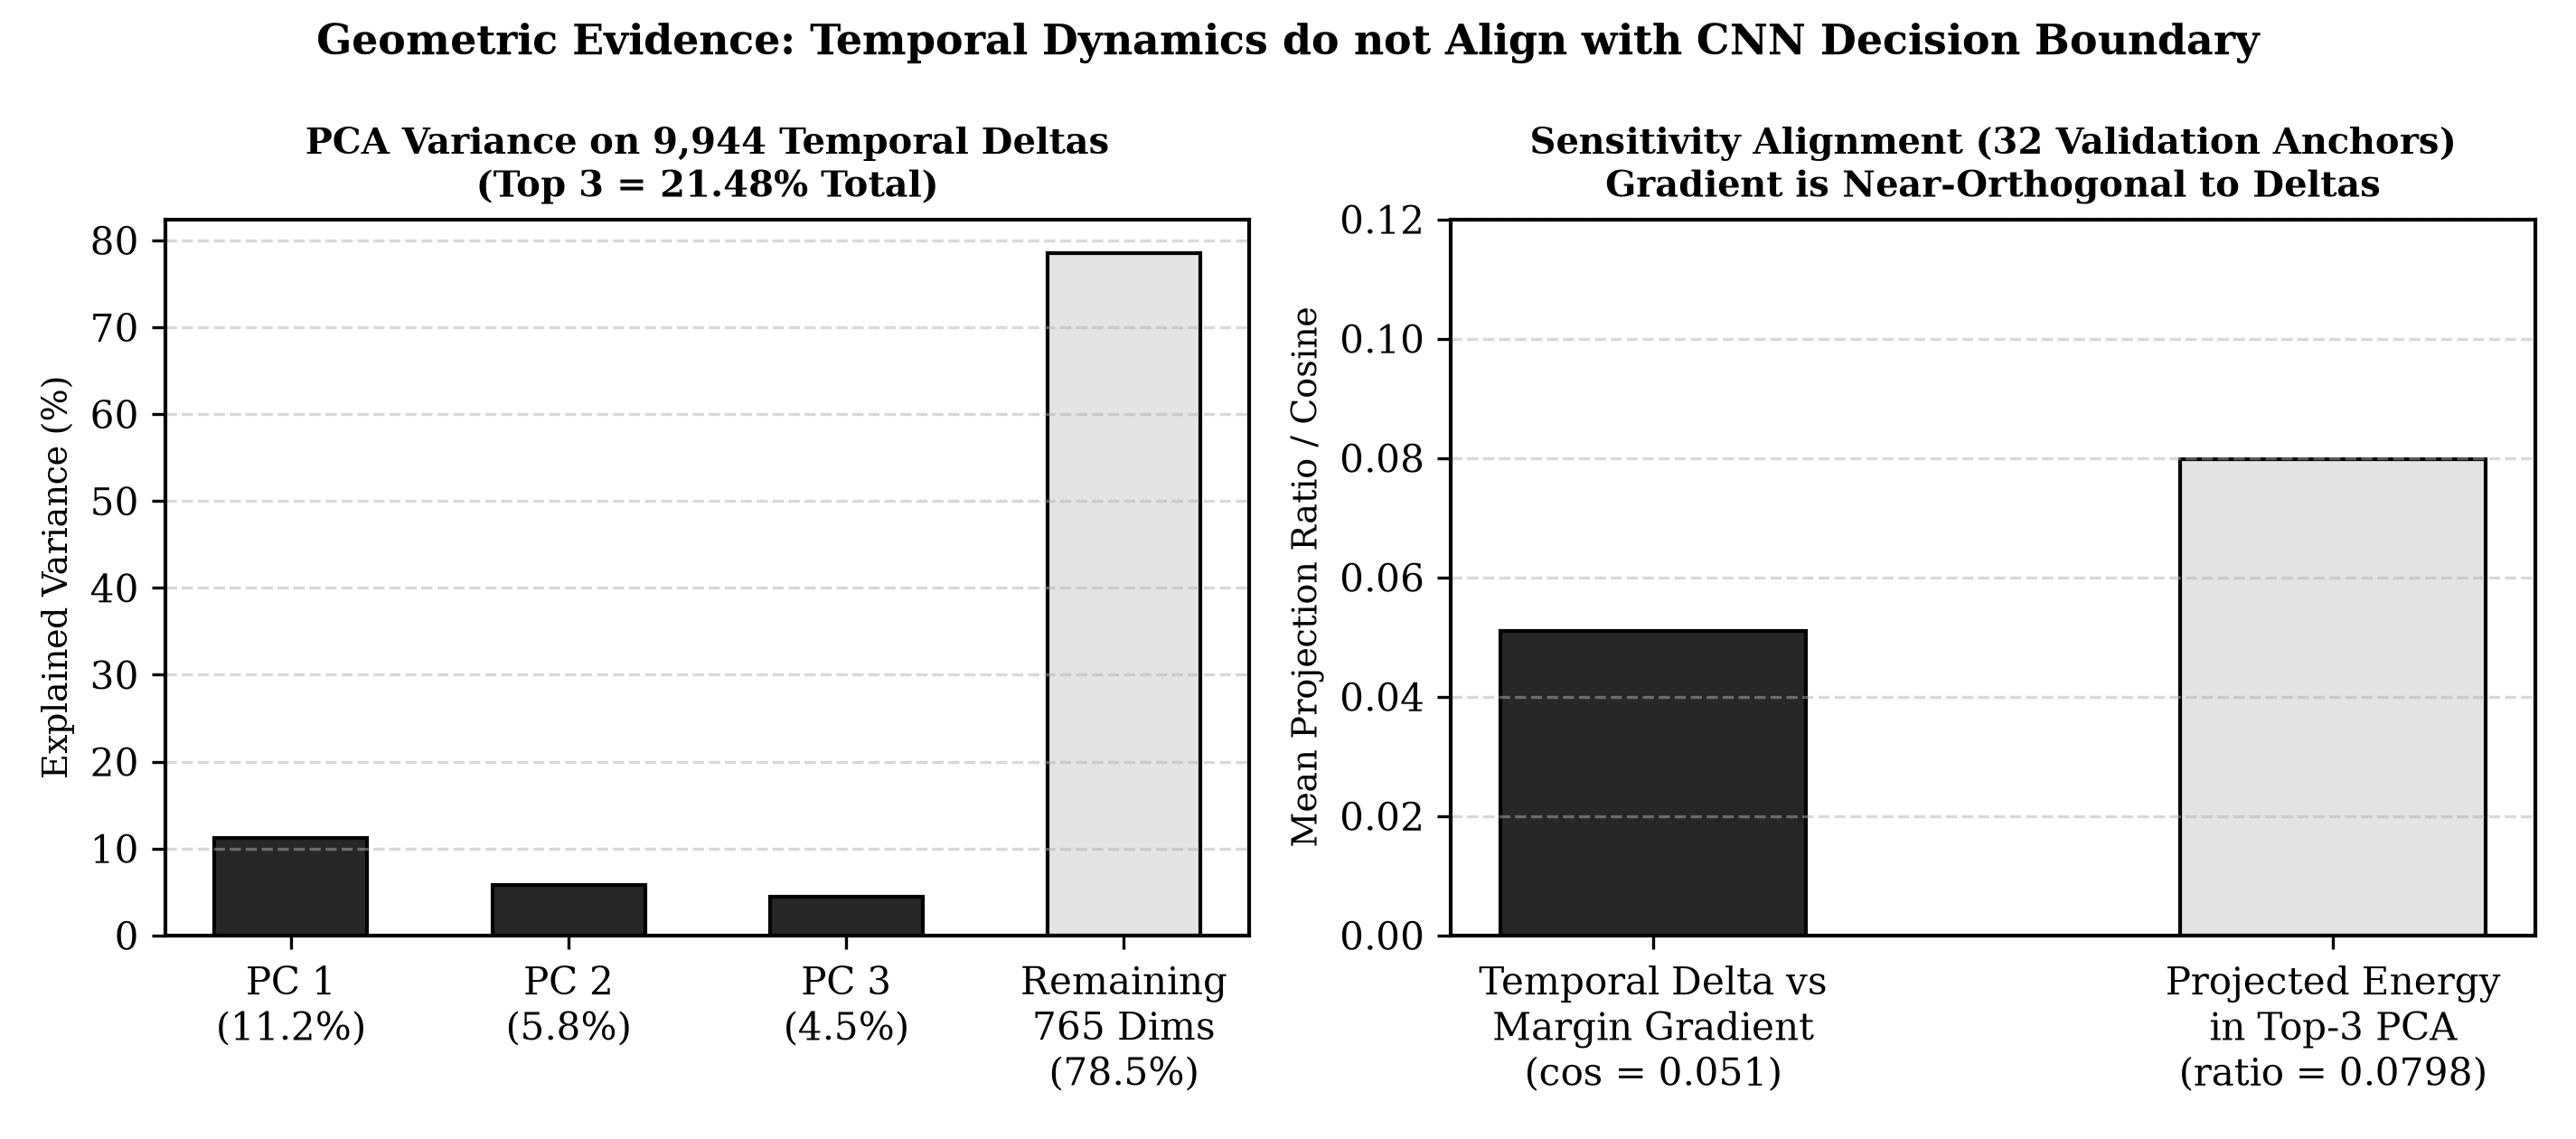
\includegraphics[width=\textwidth]{assets/fig06_geometry_pca_gradient.png}
        \end{column}
        \begin{column}{0.42\textwidth}
            \begin{block}{\textbf{Đo Đạc Hình Học Cụ Thể}}
                \footnotesize
                \begin{itemize}
                    \item \textbf{9.944 train deltas:} 3 trục PCA đầu chỉ chiếm \textbf{21,48\%} tổng phương sai.
                    \item \textbf{32 validation gradients:} Cosine giữa biến thiên thời gian và gradient margin chỉ đạt \textbf{0,051} (gần như vuông góc 87°).
                \end{itemize}
            \end{block}
            \vspace{0.1cm}
            \footnotesize
            Biến thiên cảm biến phân tán đa chiều và không trùng hướng nhạy cảm của CNN!
        \end{column}
    \end{columns}
\end{frame}

% SLIDE 16: RADIUS DILEMMA
\begin{frame}{Nghịch Lý Bán Kính: Cận Margin vs Membership}{Part D. Experimental Methodology • Slide 16}
    \begin{columns}
        \begin{column}{0.55\textwidth}
            \centering
            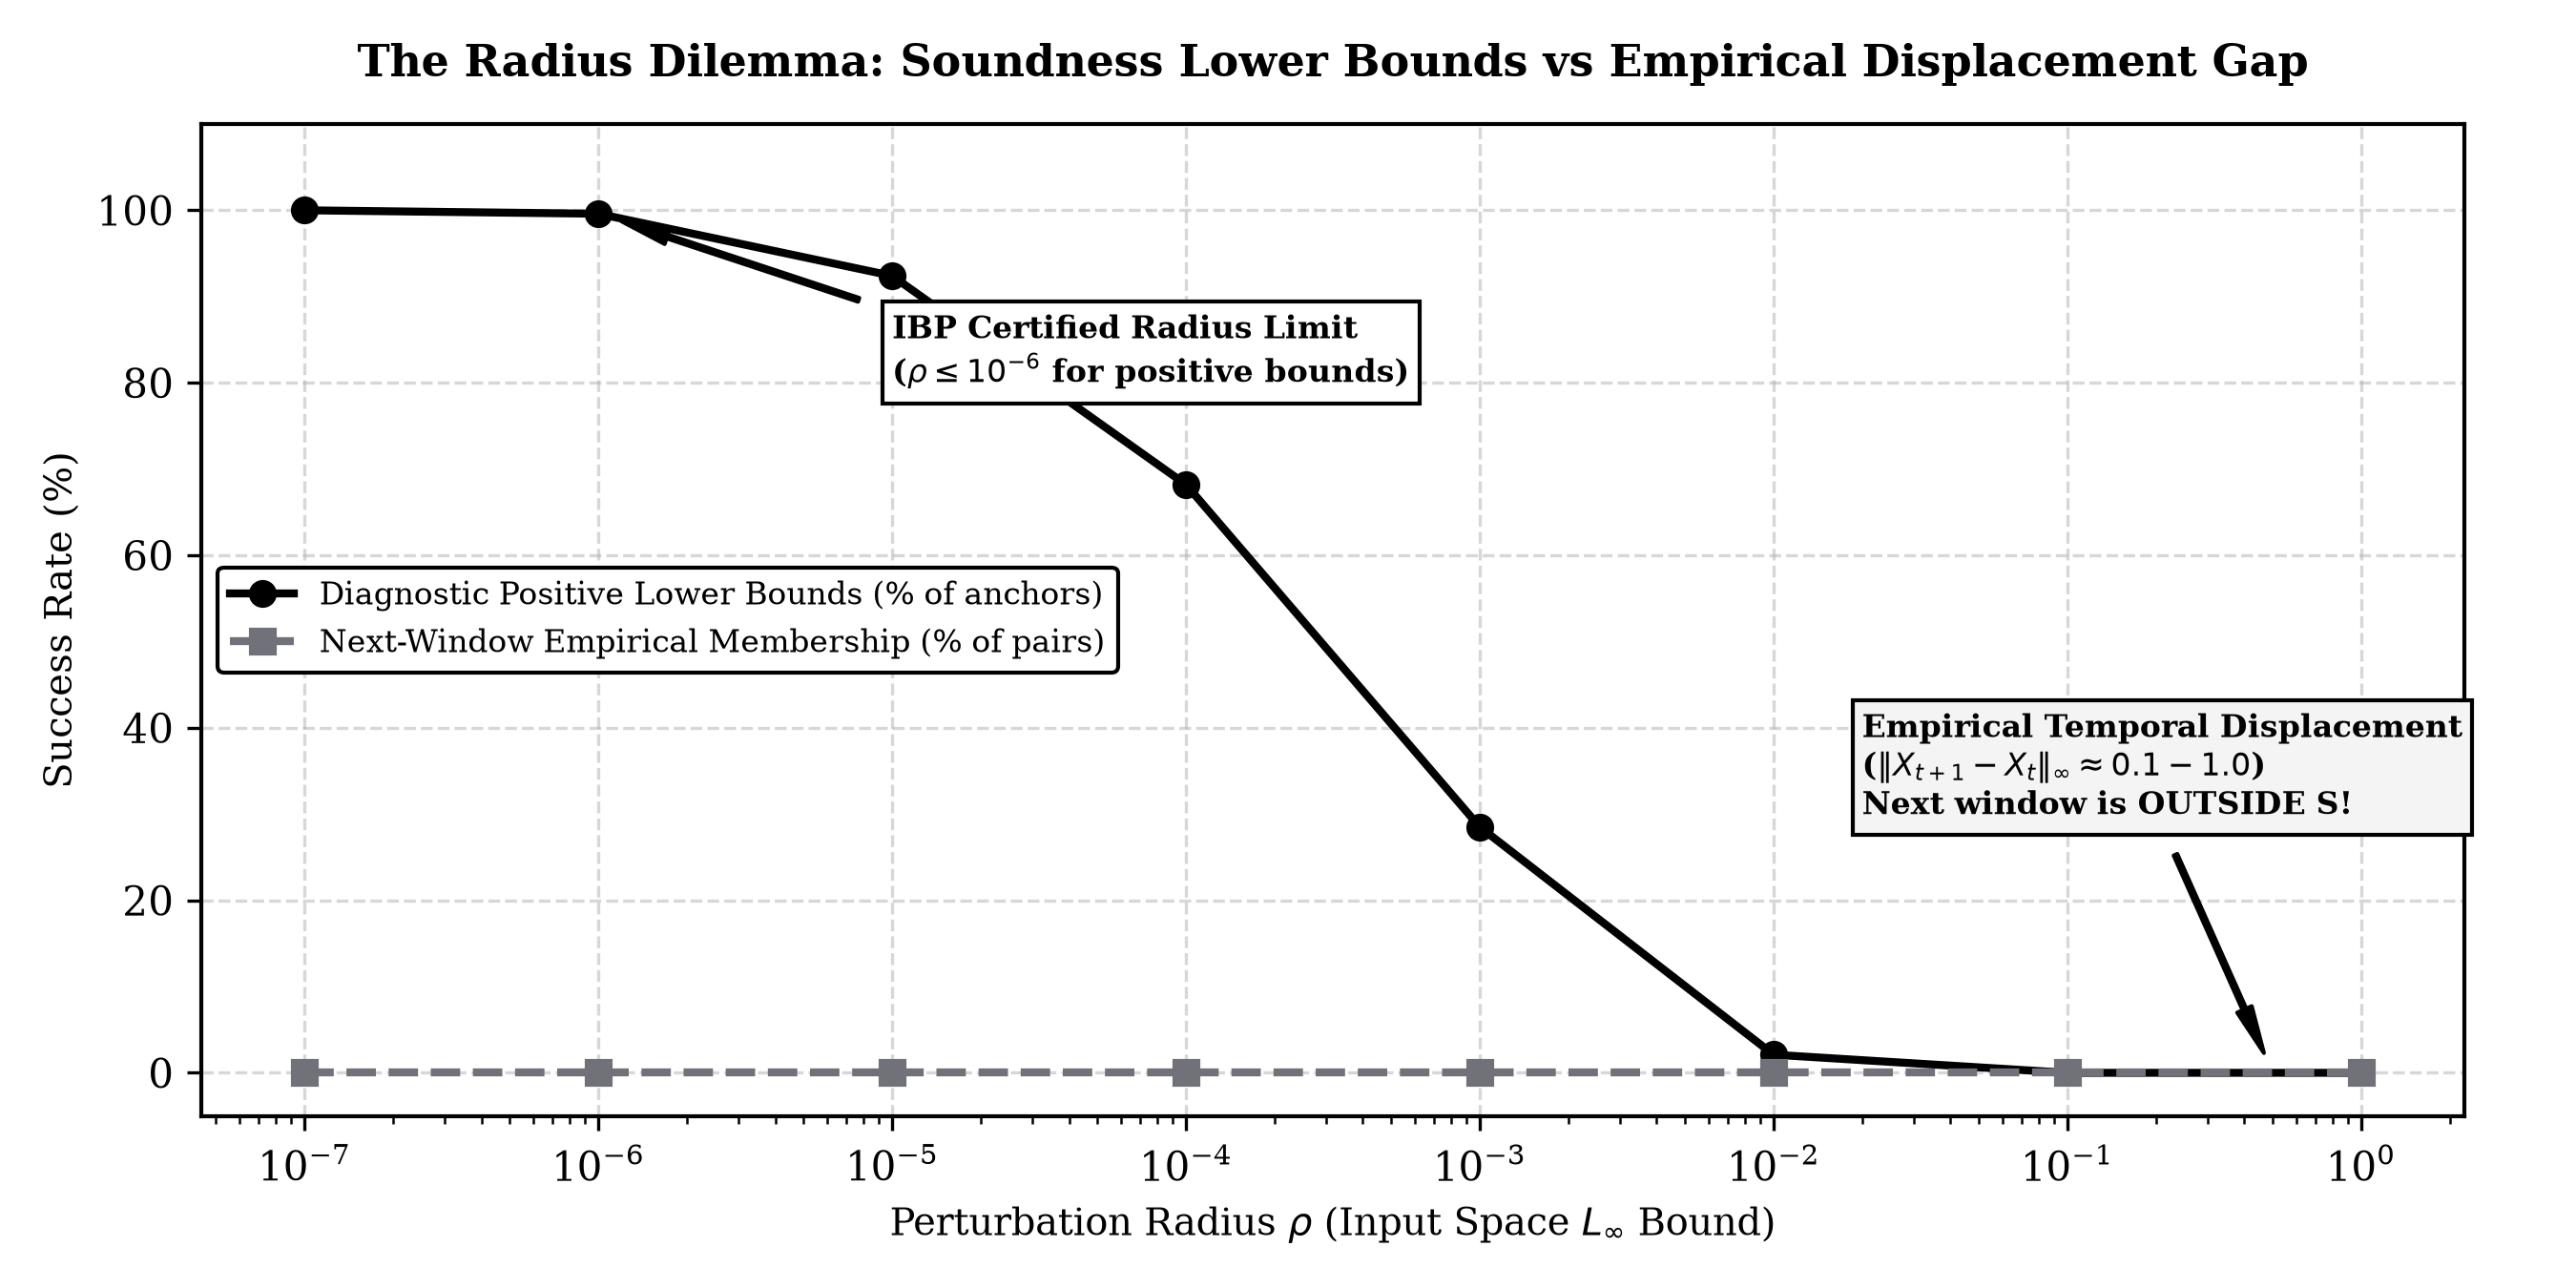
\includegraphics[width=\textwidth]{assets/fig04_radius_dilemma.png}
        \end{column}
        \begin{column}{0.42\textwidth}
            \begin{alertblock}{\textbf{Kết Quả Trên 5.053 Cửa Sổ Test}}
                \footnotesize
                \begin{itemize}
                    \item \textbf{Box Positive Builds:} 5.034 (99,6\%).
                    \item \textbf{Wave Positive Builds:} 4.211 (83,3\%).
                    \item \textbf{Next-window Members:} \textbf{0 (0,0\%)}.
                    \item \textbf{Accepted Reuse:} \textbf{0 (0,0\%)}.
                \end{itemize}
            \end{alertblock}
            \footnotesize
            \textbf{Nghịch lý:} Bán kính nhỏ thì giữ được cận dương nhưng miền rỗng; bán kính lớn để chứa dữ liệu thì cận margin bị âm do over-approximation!
        \end{column}
    \end{columns}
\end{frame}

% SLIDE 17: RUNTIME REPLAY
\begin{frame}{Kết Quả Replay Thực Tế: 20.212 Lượt Truy Vấn}{Part E. Findings, Costs \& Verification • Slide 17}
    \small
    \begin{tabular}{lcccc}
        \toprule
        \textbf{Thông số Replay} & \textbf{Run 0: Box} & \textbf{Run 0: Wave} & \textbf{Run 1: Box} & \textbf{Run 1: Wave} \\
        \midrule
        Tổng số cửa sổ test & 5.053 & 5.053 & 5.053 & 5.053 \\
        Số lần build runtime & 49 & 69 & 49 & 69 \\
        Số lần build positive & 48 & 48 & 48 & 48 \\
        \textbf{Accepted reuse queries} & \textcolor{AlertRed}{\textbf{0}} & \textcolor{AlertRed}{\textbf{0}} & \textcolor{AlertRed}{\textbf{0}} & \textcolor{AlertRed}{\textbf{0}} \\
        \textbf{Tỷ lệ Fallback về CNN} & \textcolor{AlertRed}{\textbf{100,0\%}} & \textcolor{AlertRed}{\textbf{100,0\%}} & \textcolor{AlertRed}{\textbf{100,0\%}} & \textcolor{AlertRed}{\textbf{100,0\%}} \\
        \textbf{Disagreements với Reference} & \textcolor{MintGreen}{\textbf{0}} & \textcolor{MintGreen}{\textbf{0}} & \textcolor{MintGreen}{\textbf{0}} & \textcolor{MintGreen}{\textbf{0}} \\
        \bottomrule
    \end{tabular}
    \vspace{0.3cm}
    \begin{alertblock}{\textbf{Cảnh Báo Về Số Liệu 0 Disagreements}}
        Con số 0 Disagreements xuất hiện vì \textbf{100\% truy vấn đều fallback về CNN}, không phải vì chứng chỉ hoạt động thành công! Accuracy trên reused queries là \textbf{N/A}.
    \end{alertblock}
\end{frame}

% SLIDE 18: COST BREAKDOWN
\begin{frame}{Đo Đạc Chi Phí: ECDR Có Tiết Kiệm Không?}{Part E. Findings, Costs \& Verification • Slide 18}
    \begin{columns}
        \begin{column}{0.55\textwidth}
            \centering
            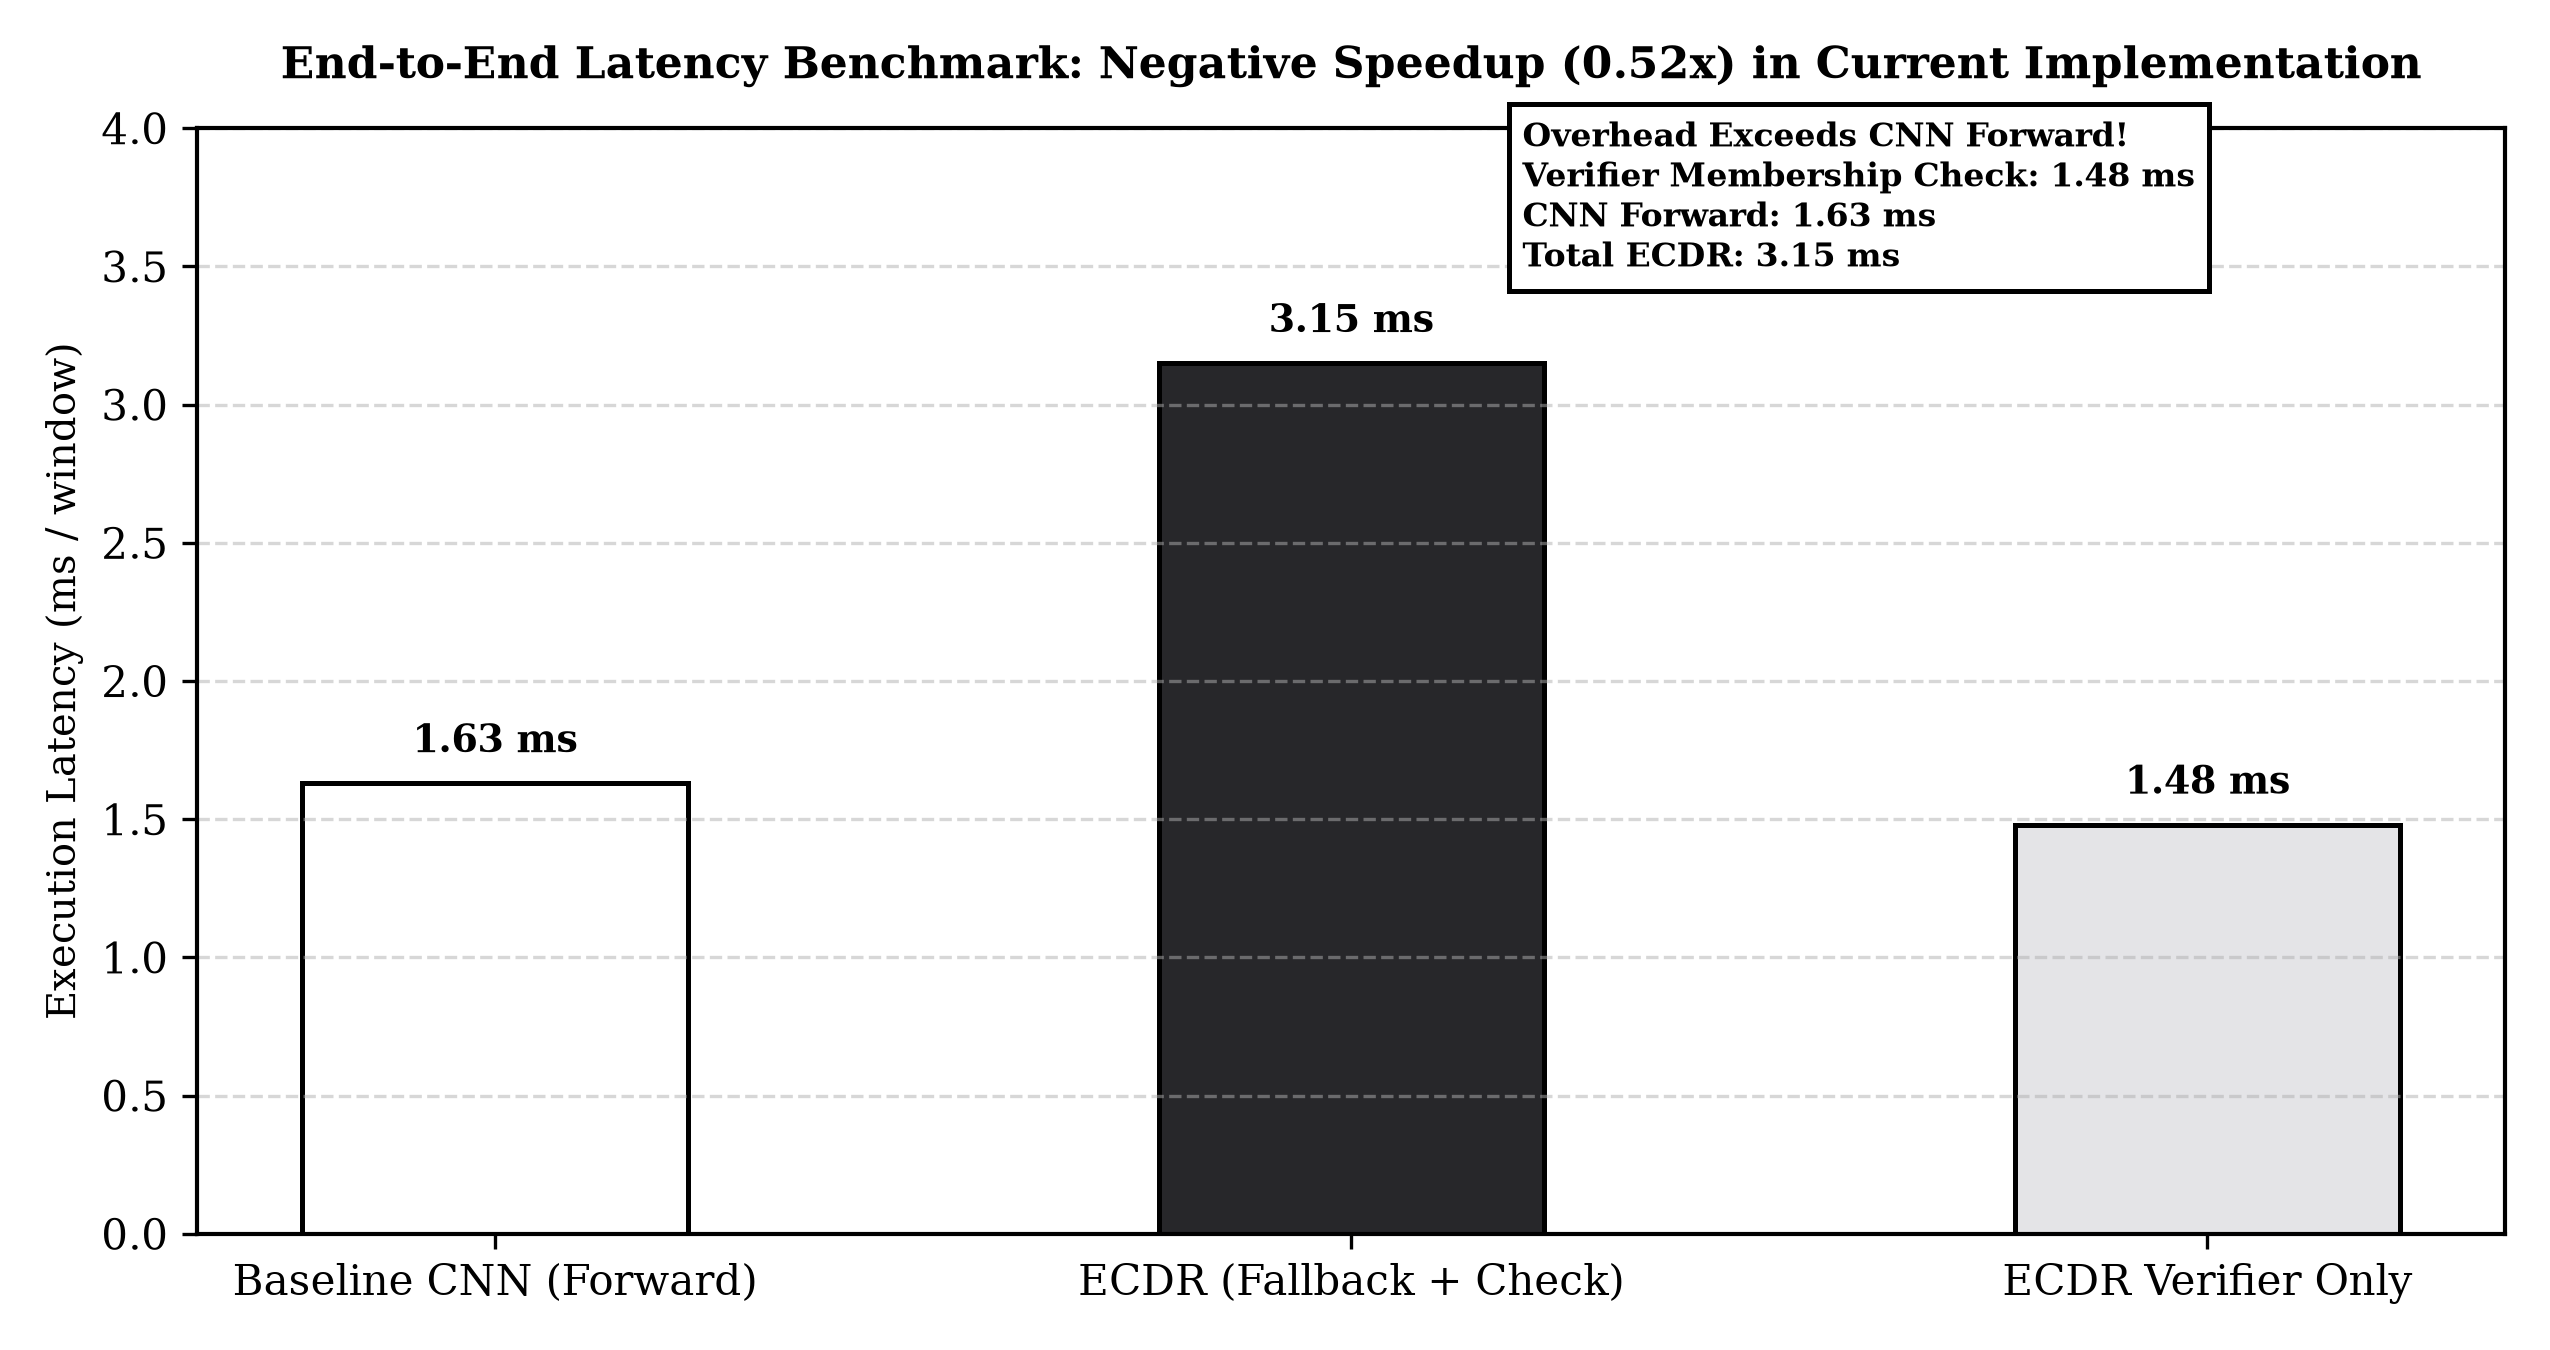
\includegraphics[width=\textwidth]{assets/fig05_latency_comparison.png}
        \end{column}
        \begin{column}{0.42\textwidth}
            \begin{block}{\textbf{Mô Hình Chi Phí Hòa Vốn}}
                \footnotesize
                $$T_{\text{ECDR}} \approx T_e + T_m + (1-r)T_f + q T_b$$
                Điều kiện có lãi: $r T_f > T_e + T_m + q T_b$.
                \begin{itemize}
                    \item $T_m$ (check membership): $\sim 1,43$ ms.
                    \item $T_f$ (full fallback): $\sim 1,67$ ms.
                    \item $r = 0 \implies$ Tiết kiệm ròng luôn \textbf{ÂM}!
                \end{itemize}
            \end{block}
            \vspace{0.1cm}
            Tốc độ tương đối hiện tại: $\sim \mathbf{0,52\times}$ (chậm gấp đôi baseline).
        \end{column}
    \end{columns}
\end{frame}

% SLIDE 19: MEMORY FOOTPRINT
\begin{frame}{Dung Lượng Bộ Nhớ \& Thành Phần Vận Hành}{Part E. Findings, Costs \& Verification • Slide 19}
    \begin{columns}
        \begin{column}{0.55\textwidth}
            \centering
            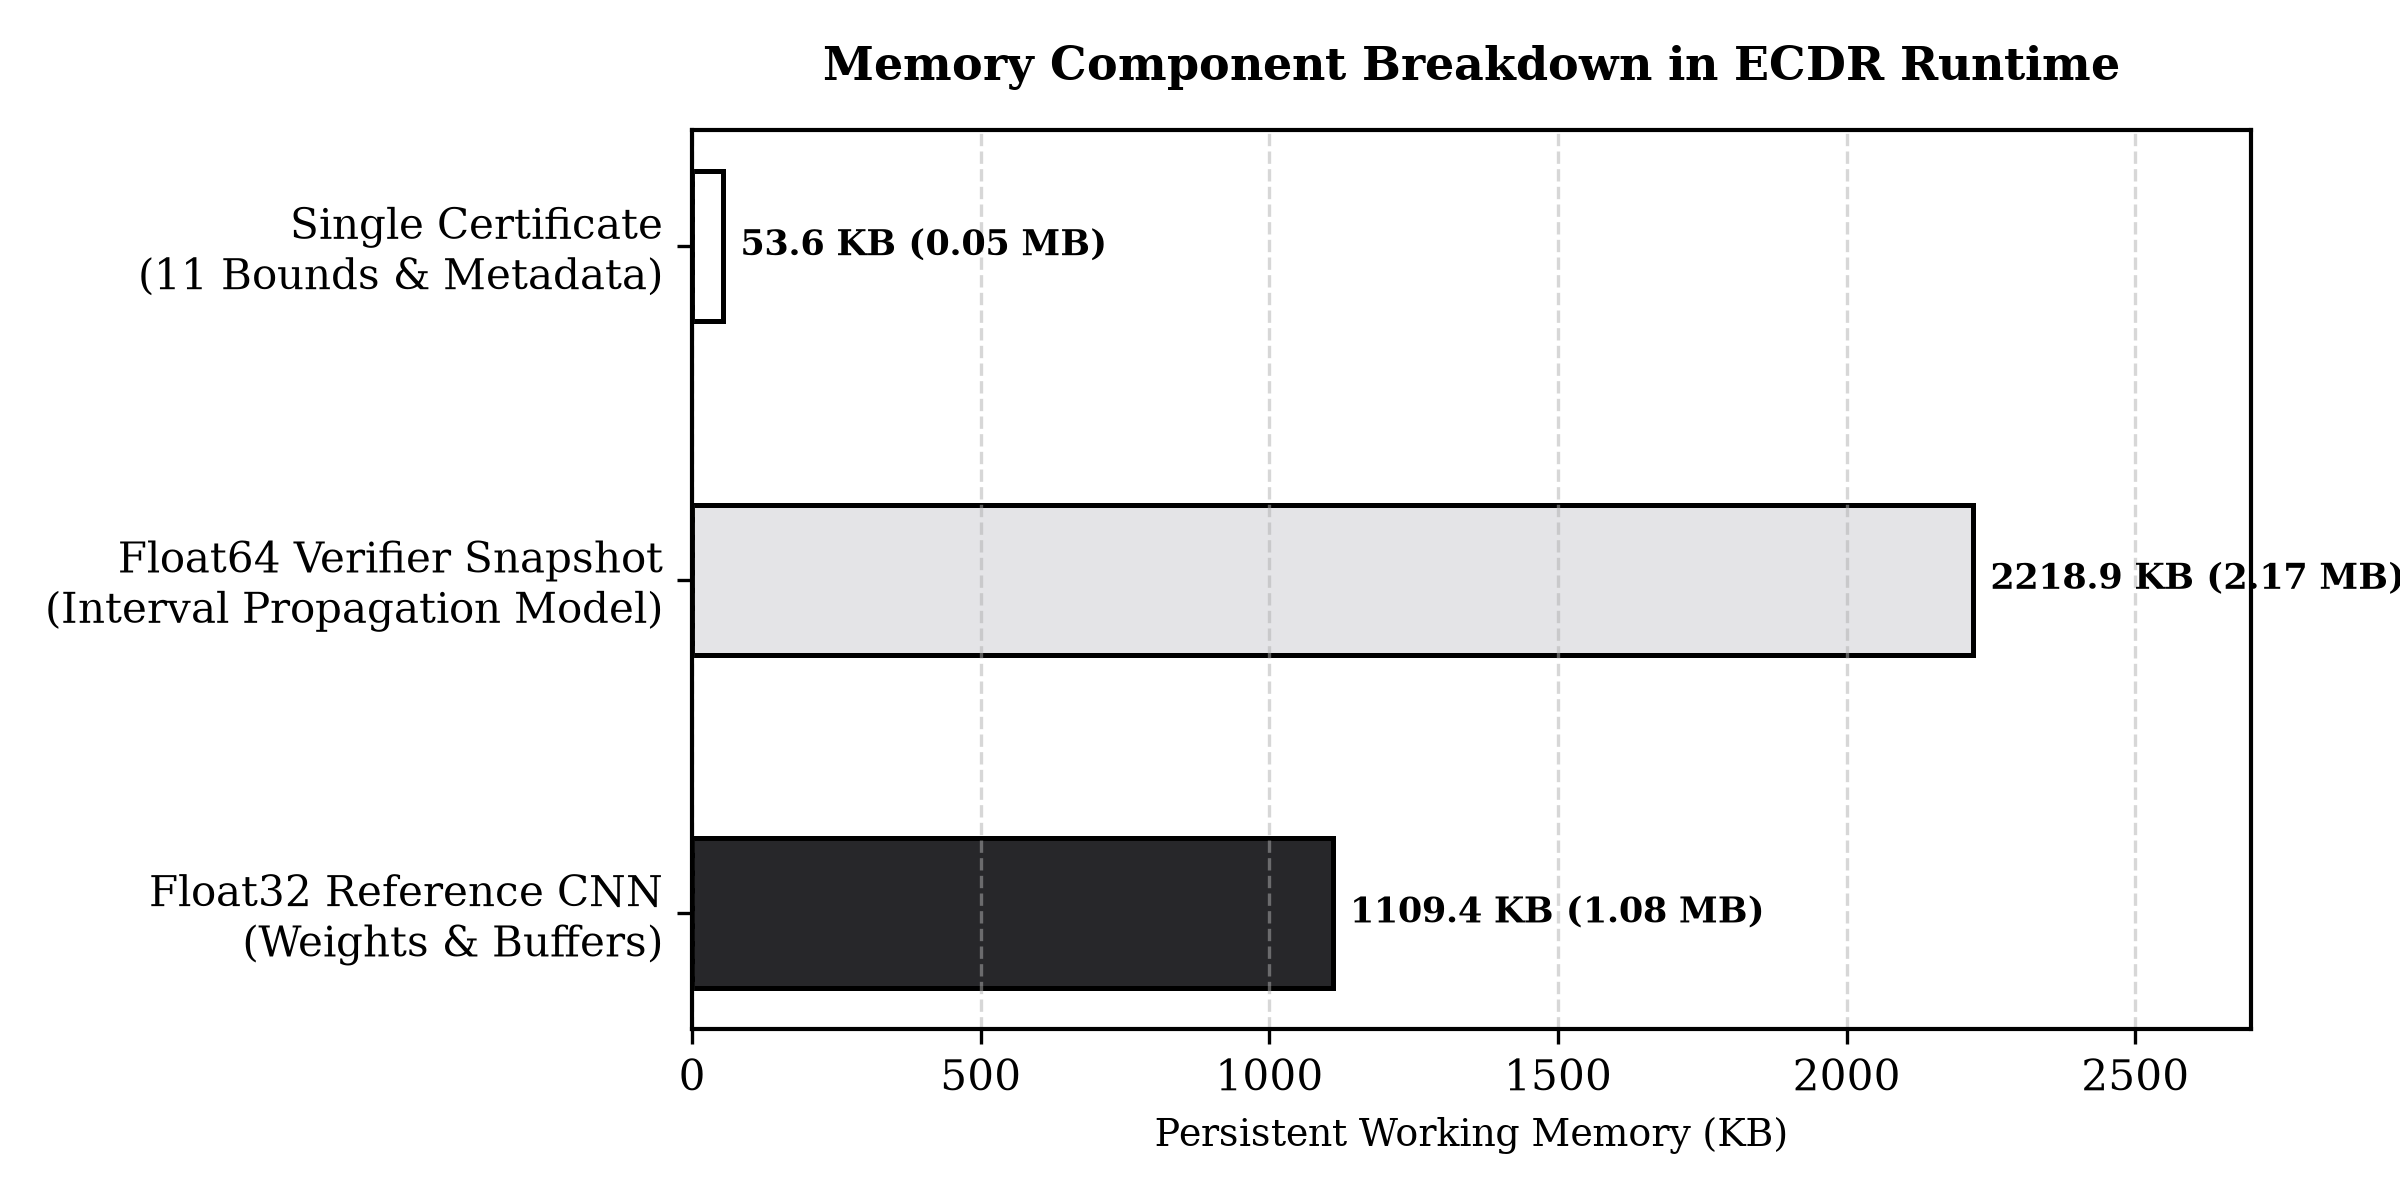
\includegraphics[width=\textwidth]{assets/fig08_memory_breakdown.png}
        \end{column}
        \begin{column}{0.42\textwidth}
            \begin{block}{\textbf{Phân Rã Bộ Nhớ Thực Tế}}
                \footnotesize
                \begin{itemize}
                    \item \textbf{Reference Float32:} 1.136.072 bytes ($\sim 1,14$ MB) cho weights và buffers.
                    \item \textbf{Verifier Float64:} 2.272.120 bytes ($\sim 2,27$ MB) snapshot IBP.
                    \item \textbf{Conditional Certificate:} 54.839 bytes ($\sim 54,8$ KB) bộ nhớ Python.
                \end{itemize}
            \end{block}
            \vspace{0.1cm}
            \footnotesize
            Bộ nhớ working memory hoàn toàn nằm trong giới hạn cho phép của thiết bị nhúng.
        \end{column}
    \end{columns}
\end{frame}

% SLIDE 20: SCIENTIFIC FINDINGS
\begin{frame}{Phát Hiện Khoa Học \& Chuỗi Nguyên Nhân Gốc}{Part E. Findings, Costs \& Verification • Slide 20}
    \begin{columns}
        \begin{column}{0.48\textwidth}
            \begin{block}{\textbf{3 Nhóm Phát Hiện Khoa Học}}
                \footnotesize
                \begin{enumerate}
                    \item \textbf{Đã Thiết Lập:} Cận margin dương bảo toàn winner giải tích; Feature alignment khớp bitwise 100\%.
                    \item \textbf{Chưa Đạt:} Chưa có numerical bridge float32; Chưa có accepted reuse.
                    \item \textbf{Kết Quả Tiêu Cực:} Net savings âm; tốc độ chậm hơn baseline.
                \end{enumerate}
            \end{block}
        \end{column}
        \begin{column}{0.48\textwidth}
            \begin{alertblock}{\textbf{Hai Rào Cản Độc Lập (Blockers)}}
                \footnotesize
                \begin{itemize}
                    \item \textbf{Blocker A (Số học):} Cận float64 chưa bao bọc float32 $\implies$ khóa formal reuse.
                    \item \textbf{Blocker B (Thể tích):} Nghịch lý bán kính $\implies$ 0 next members.
                \end{itemize}
            \end{alertblock}
            \vspace{0.1cm}
            \textbf{Trạng thái Gates:} G2 HOLD, G3 PARTIAL, G4/G5/G6 NOT ACHIEVED.
        \end{column}
    \end{columns}
\end{frame}

% SLIDE 21: VERIFICATION & HANDOFF
\begin{frame}{Thẩm Định Tính Tái Lập \& Bàn Giao Tuần 4}{Part E. Findings, Costs \& Verification • Slide 21}
    \begin{columns}
        \begin{column}{0.48\textwidth}
            \begin{block}{\textbf{Bằng Chứng Tái Lập}}
                \footnotesize
                \begin{itemize}
                    \item \textbf{93 / 93 Tests PASS} trong 1,685 giây (60 lịch sử + 33 mới).
                    \item \textbf{26 / 26 Delivery Checks PASS}.
                    \item \textbf{170 Files} bảo vệ nguyên vẹn.
                \end{itemize}
            \end{block}
            \alert{\textbf{Lưu ý:}} Test pass $\neq$ G3 pass!
        \end{column}
        \begin{column}{0.48\textwidth}
            \begin{block}{\textbf{Kế Hoạch Ưu Tiên Tuần 4}}
                \footnotesize
                \begin{itemize}
                    \item \textbf{[P0] Numerical-soundness bridge:} Xây dựng interval directed rounding cho float32.
                    \item \textbf{[P0] Revisit candidate domain:} Thiết kế miền dynamic/adaptive để đón next windows.
                    \item \textbf{[P1] CROWN \& LipCache:} Benchmark so sánh công bằng trên cùng ranh giới kế toán.
                \end{itemize}
            \end{block}
        \end{column}
    \end{columns}
\end{frame}

% SLIDE 22: DASHBOARD
\begin{frame}{Bảng Điều Khiển Quản Trị Dự Án Tuần 3 (Dashboard)}{Part F. Project Management • Slide 22}
    \tiny
    \begin{tabular}{lp{6cm}c}
        \toprule
        \textbf{Tiêu chí Tutor} & \textbf{Nội dung chi tiết Tuần 3} & \textbf{Trạng thái} \\
        \midrule
        \textbf{1. WHAT} & 2 Báo cáo Toán học (59p), Verifier actual K=12, bộ 93 tests, bộ dữ liệu 5.053 cửa sổ. & \textcolor{MintGreen}{\textbf{Hoàn thành}} \\
        \textbf{2. WHEN} & Toàn bộ thí nghiệm và receipts hoàn tất ngày 03/11/2026. & \textcolor{MintGreen}{\textbf{Đạt mốc}} \\
        \textbf{3. WHY} & Kiểm chứng tính khả thi thực thi của chứng nhận toán học và đo chi phí suy luận. & \textcolor{MintGreen}{\textbf{Mục tiêu rõ ràng}} \\
        \textbf{4. WHO} & Phân công: Toán lý thuyết, Lập trình verifier, Thực nghiệm, Kiểm thử độc lập. & \textcolor{WarnAmber}{\textbf{Cần confirm}} \\
        \textbf{5. HOW MUCH} & Phân biệt rõ: Thời gian máy chạy (1,68s tests + 168s replay) KHÔNG PHẢI giờ làm việc kỹ sư. & \textcolor{WarnAmber}{\textbf{Cần Timesheet}} \\
        \textbf{6. TOP RISKS} & Gate G2 HOLD, rủi ro sai số số học float32 (G3), miền ứng viên không chứa dữ liệu (G4). & \textcolor{AlertRed}{\textbf{Đã định lượng}} \\
        \textbf{7. MAJOR CHANGES} & Chuyển hoàn toàn từ K=6/GAP sang K=12/Flatten-MLP trên đồ thị thật; khóa bằng SHA256. & \textcolor{MintGreen}{\textbf{Khóa SHA256}} \\
        \textbf{8. KEY ISSUES} & Reuse = 0\%, tiết kiệm ròng âm, auto-LiRPA xung đột phiên bản với PyTorch 2.14. & \textcolor{AlertRed}{\textbf{Phân tích xong}} \\
        \bottomrule
    \end{tabular}
\end{frame}

% SLIDE 23: APPENDIX HYPOTHESIS MATRIX
\begin{frame}{Phụ Lục 1: Ma Trận 24 Giả Thuyết (H01–H24)}{Appendix • Slide 23}
    \tiny
    \begin{tabular}{llll|llll}
        \toprule
        \textbf{ID} & \textbf{Nội dung} & \textbf{Trạng thái} & \textbf{Bằng chứng} & \textbf{ID} & \textbf{Nội dung} & \textbf{Trạng thái} & \textbf{Bằng chứng} \\
        \midrule
        H01 & Shift overlap equality & \textcolor{MintGreen}{DERIVED} & Stride 64 & H13 & Feature alignment & \textcolor{MintGreen}{DERIVED} & 3.866.112 checks \\
        H02 & Overlap $\implies$ small dist & \textcolor{AlertRed}{FALSIFIED} & Counterex & H14 & GAP feature sum & \textcolor{AlertRed}{FALSIFIED} & Không áp cho MLP \\
        H03 & Same label $\implies$ same pred & \textcolor{AlertRed}{FALSIFIED} & Witness 682-683 & H15 & Recenter no proof & \textcolor{AlertRed}{FALSIFIED} & Drift rủi ro \\
        H04 & Local invariant region & \textcolor{MintGreen}{DERIVED} & Liên tục & H16 & Fixed-anchor reuse & \textcolor{WarnAmber}{CONDITIONAL} & Cần valid bounds \\
        H05 & Positive margin bounds & \textcolor{MintGreen}{DERIVED} & Định lý cốt lõi & H17 & Multi-step wave & \textcolor{WarnAmber}{CONDITIONAL} & Reachable bounds \\
        H06 & Lipschitz ball & \textcolor{WarnAmber}{CONDITIONAL} & Cần hằng số L & H18 & Box membership & \textcolor{MintGreen}{DERIVED} & $\Theta(m)$ \\
        H07 & IBP always certifies & \textcolor{AlertRed}{FALSIFIED} & Incomplete & H19 & Sound $\implies$ coverage & \textcolor{AlertRed}{FALSIFIED} & Miền có thể rỗng \\
        H08 & Direct pairwise margin & \textcolor{MintGreen}{DERIVED} & Giảm loss & H20 & Coverage $\implies$ speed & \textcolor{AlertRed}{FALSIFIED} & Overhead triệt tiêu \\
        H09 & CROWN cheaper & \textcolor{gray}{NOT ESTAB} & Chưa chứng & H21 & ECDR beats LipCache & \textcolor{gray}{NOT ESTAB} & Thiếu benchmark \\
        H10 & PCA matches gradient & \textcolor{gray}{DESCRIPTIVE} & Cosine 0,051 & H22 & Real $\implies$ float32 & \textcolor{AlertRed}{FALSIFIED} & Sai số làm tròn \\
        H11 & Structured beats box & \textcolor{gray}{NOT ESTAB} & Chưa chứng & H23 & Event name is enough & \textcolor{AlertRed}{FALSIFIED} & Cần margin bounds \\
        H12 & Overlap 768 $\to$ 384 & \textcolor{MintGreen}{DERIVED} & Hình học & H24 & Sound + saving regime & \textcolor{gray}{NOT ESTAB} & Chưa đạt \\
        \bottomrule
    \end{tabular}
\end{frame}

% SLIDE 24: APPENDIX RUBRIC MAPPING
\begin{frame}{Phụ Lục 2: Đối Chiếu Rubric Đánh Giá Đặc Thù Của Tutor}{Appendix • Slide 24}
    \small
    \begin{tabular}{lp{6cm}p{3.5cm}}
        \toprule
        \textbf{Tiêu chí Rubric} & \textbf{Nội dung phản ánh trong Slide} & \textbf{Bằng chứng Repository} \\
        \midrule
        \textbf{Data Preparation} & Khóa tập Train/Val/Test của HAPT; bảng chuẩn hóa Z-score lưu trữ bằng SHA256. & Slide 02, 05 \\
        \textbf{Feature Engineering} & 768 tọa độ raw, căn chỉnh feature maps 12 vị trí (H13), phân tích không gian PCA 21,5\%. & Slide 05, 09, 15 \\
        \textbf{Model Selection} & Khóa SmallCNN1D 283.692 params; giải thích sự cần thiết của verifier trên đồ thị thật. & Slide 02, 07, 11 \\
        \textbf{Baseline Metrics} & Xác minh 100\% khớp predictions trên 5.053 cửa sổ test; đo latency trên CPU single-thread. & Slide 02, 17, 18 \\
        \textbf{Planned Tasks} & Lộ trình P0 (Numerical bridge, candidate domain redesign) và P1 (CROWN, overhead reduction). & Slide 21 \\
        \bottomrule
    \end{tabular}
\end{frame}

\end{document}
